% ------------ begin cheatsheet

\documentclass[a4paper]{article}
\usepackage[a4paper,margin=0.17in,landscape]{geometry}
\usepackage{multicol}

\usepackage{amsmath, amssymb}
\usepackage{enumitem}
\usepackage{graphicx}

\usepackage{ulem}
\usepackage{makecell}

% math
\newcommand{\abs}[1]{\left\lvert#1\right\rvert}

% envs
\newcommand{\ol}[1]{\begin{enumerate}#1\end{enumerate}}
\newcommand{\oll}[1]{\begin{enumerate}[leftmargin=*]#1\end{enumerate}}
\newcommand{\ul}[1]{\begin{itemize}#1\end{itemize}}
\newcommand{\ull}[1]{\begin{itemize}[leftmargin=*]#1\end{itemize}}

\graphicspath{ {./images/} }
\pagestyle{empty}
\setlength{\columnseprule}{0.3pt}

% reduce spacing before and after headers
\newcommand{\uppercaseandunderline}[1]{\uline{\uppercase{#1}}}

\makeatletter
\renewcommand{\section}{
	\@startsection{section}{1}{0pt}{1ex}{1.2ex} {\raggedleft\normalfont\large\bfseries\uppercaseandunderline}}
\renewcommand{\subsection}{
	\@startsection{subsection}{2}{0pt}{1ex}{1.2ex} {\raggedleft\normalfont\normalsize\bfseries\fbox}}
\renewcommand{\subsubsection}{
	\@startsection{subsubsection}{3}{0pt}{1ex}{0.8ex} {\raggedleft\normalfont\small\bfseries\uline}}
\renewcommand{\paragraph}{
	\@startsection{paragraph}{4}{0pt}{1.5ex}{-0.8em}{\normalfont\bfseries}}
% ------------ end cheatsheet

% ------------ begin code
\usepackage{xcolor}
\definecolor{dkgreen}{rgb}{0,0.6,0}
\definecolor{gray}{rgb}{0.5,0.5,0.5}
\definecolor{mauve}{rgb}{0.58,0,0.82}
\definecolor{lg}{rgb}{0.9,0.9,0.9}

% code environment
\usepackage{listings}
\lstset{
  %frame=tb, % adds top and bottom border
  aboveskip=1mm,
  belowskip=1mm,
  showstringspaces=false,
  columns=flexible,
  basicstyle={\small\ttfamily},
  numberstyle=\color{gray},
  keywordstyle=\color{blue}\textbf,
  commentstyle=\color{dkgreen},
  stringstyle=\color{mauve},
  breaklines=true,
  breakatwhitespace=true,
  backgroundcolor=\color{lg},
  tabsize=4
}
\newcommand{\ic}[1]{\lstinline{#1}}

% ------------ end code

\newcommand\tick{\item[\checkmark]}
\newcommand\cross{\item[$\times$]}

% TODO
% add next fit algo
% add quizzes

\begin{document}
\begin{multicols*}{4}
  \small
  \part*{\centering \underline{CS2106}}
\section*{Memory management} 
  \paragraph{Memory regions}
    \ull {
      \item Text (for instructions)
      \item Data (for global variables)
      \item Heap (for dynamic allocation)
      \item Stack (for function invocations)
    }
  \paragraph{Types of data}
    \ull {
      \item Transient: valid only for a limited duration (e.g. function parameters, local variables)
      \item Persistent: valid for duration of program or until explicitly deallocated (e.g. global variables, dynamically allocated memory)
    }
  \subsection*{Memory abstraction}
    \paragraph{No abstraction}
      \ull {
        \tick Address in program == physical address
        \tick No conversion/mapping required
        \tick Address fixed at compile time
        \cross Hard to protect memory space
        \cross Multiple processes might occupy same physical locations
      }
    \paragraph{Address relocation}
      \ull {
        \item Recalculate memory address at load time, so processes correctly access memory
        \cross Slow loading time
        \cross Not easy to distinguish memory reference from normal integer constant
      }
    \paragraph{Base + Limit registers}
      \ull {
        \item All memory references are compiled as an offset from the base register
        \item Compiled memory references are checked against the limit regsiter for validity
        \cross Every memory access incurs an addition and a comparison
      }
    \paragraph{Logical address}
      \ull {
        \item Is how the process views its memory space
        \item Is different from physical address, so a mapping is needed
        \item Each process has a self-contained, independent logical memory space
      }
\section*{Contiguous memory}
  \subsection*{Memory partitioning}
    \paragraph{Fixed-size partition}
      \ull {
        \item Physical memory is split into fixed number of partitions of equal size
        \item A process will occupy one of the partitions
        \tick Easy to manage
        \tick Fast to allocate, since every free partition is the same
        \tick \uline{No external fragmentation}
        \cross Partition needs to be large enough to contain the largest of processes
        \cross \underline{Internal fragmentation} occurs when process does not occupy entire partition (i.e. allocated but unused)
      }
    \paragraph{Variable-size partitions}
      \ull {
        \item Partition is created based on actual size of process
        \item OS keeps track of occupied and free regions, performing splitting and merging as necessary
        \tick Flexible, \uline{no internal fragmentation}
        \cross Need to maintain more info
        \cross Takes more time to find appropriate region
        \cross \underline{External fragmentation} occurs when there are free regions that are too small to be allocated (due to allocate/free patterns)
      }
  \subsection*{Dynamic allocation algorithms}
    \subsubsection*{Reducing external fragmentation}
      \ull {
        \item (Merging) Merge adjacent free partitions
        \item (Compaction) Move occupied partitions around to create bigger, consolidated holes
      }
    \subsubsection*{Linear search}
      \ull {
        \tick No internal fragmentation
        \cross Has external fragmentation
      }
      \paragraph{First fit} Take first hole that is large enough
      \paragraph{Best fit} Take smallest hole that is large enough
      \paragraph{Worst fit} Take largest hole
      \paragraph{Next fit} Like first fit, but upon next allocation request, resume searching from the partition where the previous allocation was performed
        \ull {
          \tick More uniform distribution of hole sizes
          \tick Faster alllocation
          \cross Needs to store an additional pointer to the place of last allocation
        }
    \subsubsection*{Buddy system}
      \begin{center}
        \begin{tabular}{ c|c }
          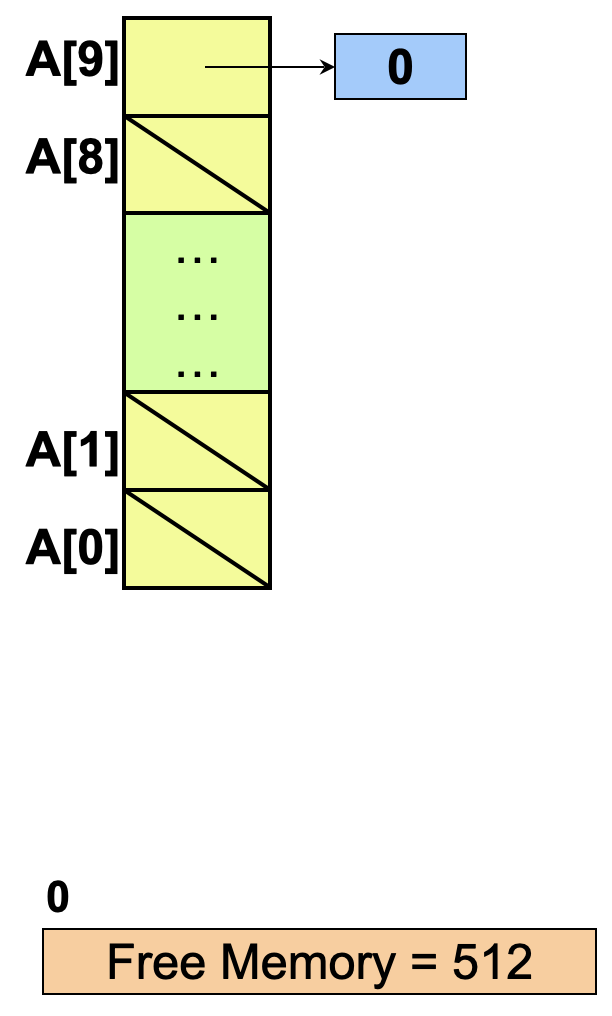
\includegraphics[height=0.12\textwidth]{buddy_before}
          &
          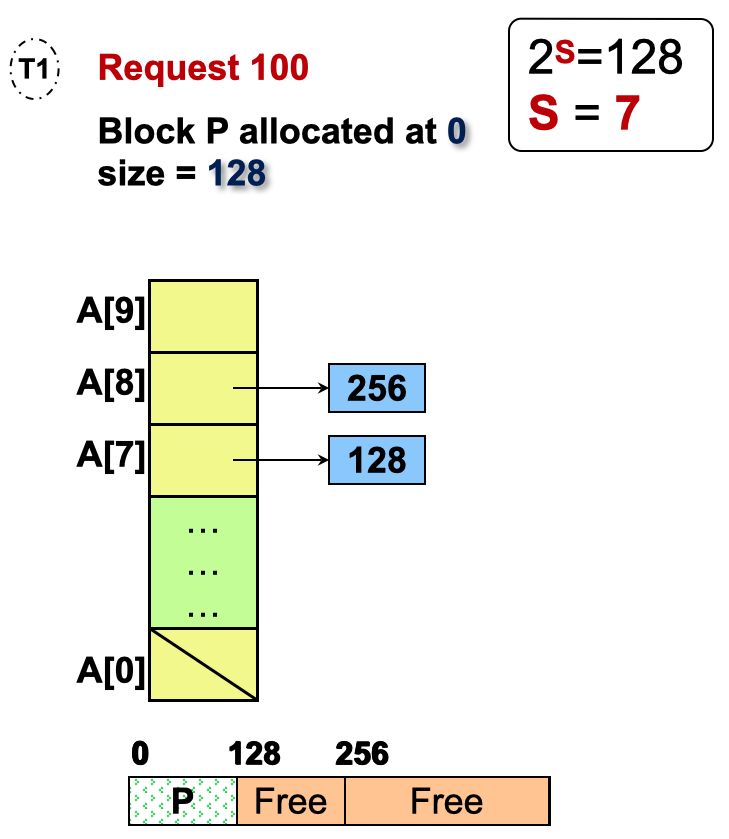
\includegraphics[height=0.12\textwidth]{buddy_after}
        \end{tabular}
      \end{center}
      Each A[i] is a list of blocks of size $2^i$, where each block indicates starting address
      \paragraph{Allocate} To allocate size $N$, find smallest $S$ such that $2^S \geq N$, then repeatedly split until there is a block of size $2^S$.
      \paragraph{Deallocate} During deallocation, if buddy is free, merge with buddy and repeat. Otherwise, add the block to the relevant linked list
      \paragraph{Check buddy} If two blocks are of size $2^S$, compare their start values. They are buddies $\iff$ only bit $S+1$ is different
      \paragraph{Fragmentation}
        \ull {
          \item Internal fragmentation (since blocks of fixed size $2^K$ are allocated, but $<50\%$)
          \item External fragmentaiton (little but possible)
        }
\section*{Disjoint memory}
  \subsection*{Paging}
    \ull {
      \item Physical memory is split into regions of fixed size (known as physical frames)
      \item Logical memory is split into regions of same size as physical frames (known as logical page)
      \item Logical memory space is contiguous, but physical memory region might be disjoint
    }
    \subsubsection*{Address translation} \noindent
      To keep things simple, frame size = page size = power of 2
      \begin{center}
        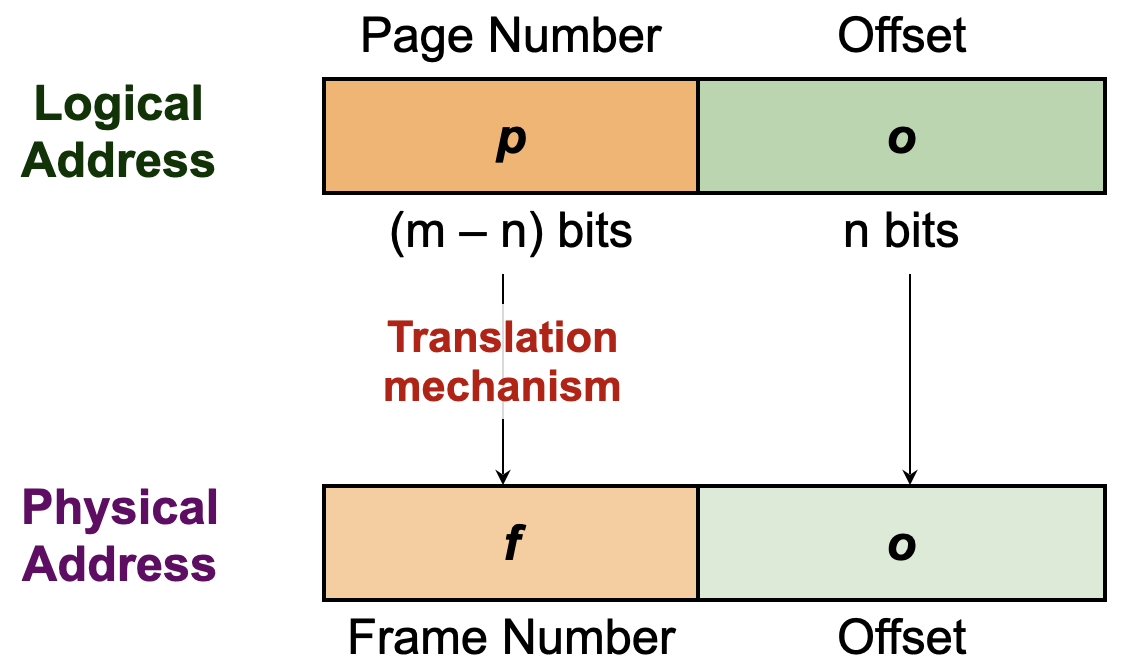
\includegraphics[width=0.2\textwidth]{page_address_translation}
      \end{center}
    \subsubsection*{Properties}
      \ull {
        \tick No external fragmentation
        \tick Can have internal fragmentation, when logical memory space is not a multiple of page size, but it is insignificant (max one page per process is not fully utilized)
        \tick Clean separation of logical and physical address space
      }
    \subsubsection*{Page table}
      \ull {
        \item Maps logical page number to physical frame number
        \item Part of process memory context (store pointer to page table)
        \cross Requires two memory accesses for each memory reference
          \ol {
            \item Get frame number from page table
            \item Access actual item
          }
      }
    \subsubsection*{Translation Look-Aside Buffer (TLB)}
      \ull {
        \item Cache for page table entries (PTEs)
        \item Very small (tens of entries) and fast ($\leq 1$ clock cycle)
        \item Not part of process hardware context
      }
      \paragraph{Memory access time}
        Let $p$ be the probability of a TLB hit.
        \begin{align*}
          \text{Latency(TLB hit)} &= \text{TLB} + \text{Mem} \\
          \text{Latency(TLB miss)} &= \text{TLB} + 2\text{Mem}
        \end{align*}
        \begin{align*}
          & \text{Average memory access time} \\
          &= p \times \text{Latency(TLB hit)} + (1-p) \times \\ 
          & \qquad \text{Latency(TLB miss)} \\
          &= p (\text{TLB} + \text{Mem}) + (1-p) (\text{TLB} + 2\text{Mem}) \\
          &= \text{TLB} + \text{Mem}(2-p)
        \end{align*}
    \subsubsection*{Protection}
      \paragraph{Access-right bits}
        \ull {
          \item Each memory access is checked against the PTE's rwx bits in hardware
        }
      \paragraph{Valid bit}
        \ull {
          \item Each memory access is checked against the valid bit in hardware
          \item Out of range access is caught by OS
        }
      \subsubsection*{Page sharing}
        \ull {
          \item Several processes might use the same physical memory frame (e.g. referencing C standard library)
          \item Can be used to implement copy-on-write
        }
  \subsection*{Segmentation}
    \subsubsection*{Motivation} \noindent
      Each memory region (text, data, heap, stack)
      \ull {
        \item May grow/shrink at execution time (hard to achieve if whole process is one piece)
        \item Hard to check if memory access in a region is in-range or not
        \item May have different usage, permissions, lifetime, scope, etc.
      }
    \subsubsection*{Idea}
      \ull {
        \item Each memory segment is a contiguous memory region, specified using \\ \ic{(segment id, base, limit)}
        \item Memory references specified as \\ \ic{(segment id, offset)}
        \item Physical address is specified using \\ \ic{(base, offset)}
        \item \ic{offset < limit} for valid access
        \cross Can cause external fragmentation
      }
  \subsection*{Segmentation with paging}
    \subsubsection*{Idea}
      \ull {
        \item Each segment has a page table, and is composed of several pages
        \item Segment can grow by allocating page and adding to page table (same for shrinking)
      }
      \begin{center}
        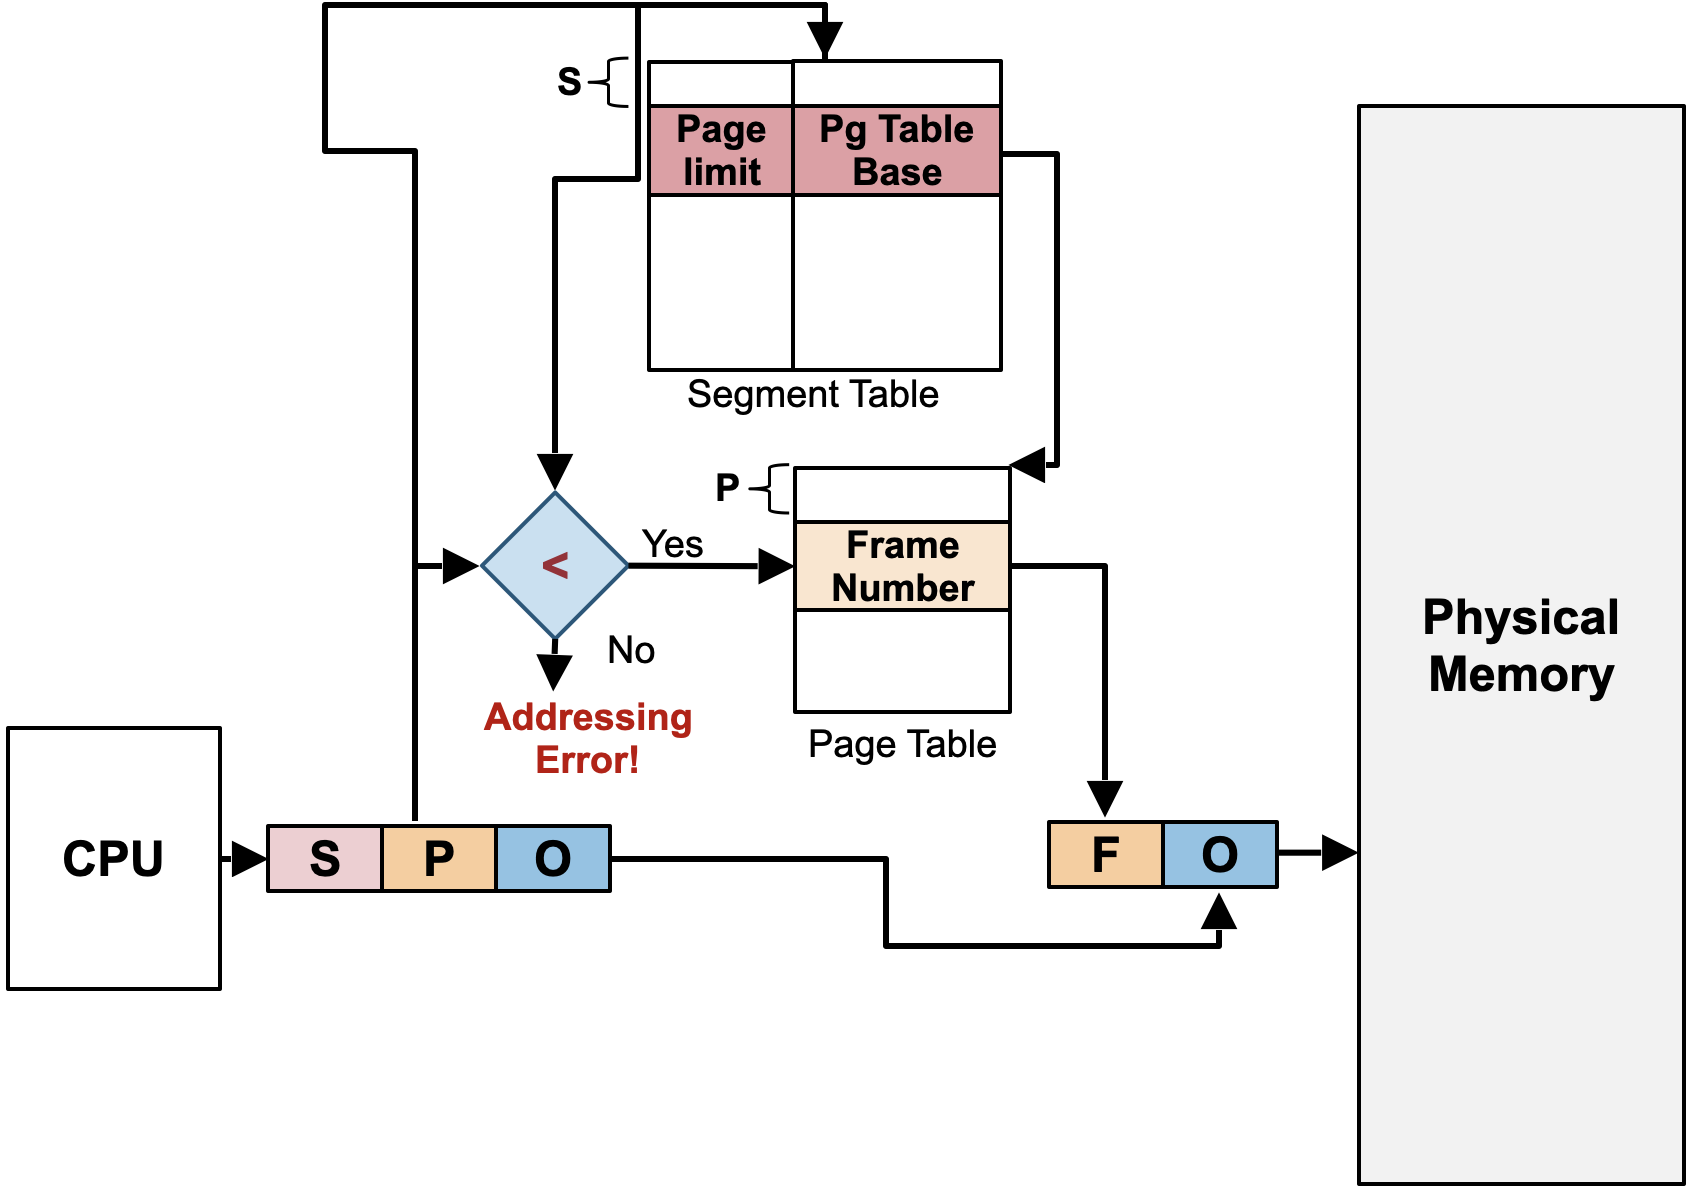
\includegraphics[width=0.24\textwidth]{segmentation_with_paging}
      \end{center}
\section*{Virtual memory}
  \subsection*{Extended paging scheme}
    \subsubsection*{Motivation} \noindent
      Logical space can be larger than physical space
    \subsubsection*{Idea}
      \ull {
        \item Split logical memory into fixed size pages
        \item Some pages are in physical memory, some in secondary storage
      }
      \paragraph{Page table} On top of storing frame number, page table entry now also needs to include resident bit - whether the page is in physical memory
      \paragraph{Page fault}
        \ull {
          \item Occurs when CPU tries to access a non-memory resident page
          \item OS needs to bring a non-memory resident page into physical memory (counts as I/O)
        }
    \subsubsection*{Issues}
      \paragraph{Secondary storage access time}
        \ull { \item 5 orders of magnitude slower than physical memory access time }
      \paragraph{Thrashing}
        \ull {
          \item Occurs when page fault happens too often
          \item Should not happen in programs that behave well, due to temporal/spatial locality
        }
  \subsection*{Access virtual address algorithm}
    \ull { \item Note: page fault counts as I/O }
    \paragraph{Algorithm for accessing VA}
      \ull { \item Done in hardware }
      \oll {
        \item VA is decomposed into \ic{<Page#, Offset>}
        \item Search TLB for \ic{<Page#>}, and if TLB miss, TRAP to OS (TLB Fault and retry algo)
        \item Is \ic{<Page#>} memory resident?, and if not, TRAP to OS (Page Fault and retry algo)
        \item Use \ic{<Frame#><Offset>} to access physical memory
      }
    \paragraph{TLB Fault Handler}
      \ull { \item Done in OS, assumes software managed TLB }
      \oll {
        \item Access full table of process (in PCB), find \ic{<Page#>}
        \item If valid bit is 0, then segmentation fault
        \item Else load relevant PTE into TLB
        \item Return from TRAP
      }
    \paragraph{TLB Fault Handler (Hardware)}
      \ull { \item Done in hardware, assumes hardware managed TLB }
      \oll {
        \item Base address of full page tabel is stored in a dedicated register
        \item Processor retrieves missing PTE from memory directly (as it is a simple offset from the base of page table)
      }
    \paragraph{Page Fault Handler}
      \ull { \item Done in OS }
      \oll {
        \item Check if global or local replacement
        \item Write out the page to be replaced if needed
        \item Locate the page in secondray storage
        \item Load the page into a physical frame
        \item Update PTE
        \item Update TLB
        \item Return from TRAP
      }
  \subsection*{Demand paging}
    \ull {
      \item Process starts with no memory resident page
      \item Only allocate page when there is a page fault
      \tick Fast startup for new process
      \tick Small memory footprint
      \cross Process may appear sluggish at the start due to multiple page faults
      \cross Page faults may have cascading effect on other processes (i.e. thrashing)
    }
  \subsection*{Page table structure} \noindent
    Assume that there are $2^P$ pages in logical memory space
    \subsubsection*{Direct paging}
      \ull {
        \item Keep all $2^P$ entries in a single table
        \cross For efficient retrieval of the $p$th entry, page tables must be contiguous in OS memory
      }
    \subsubsection*{2-level paging}
      \ull {
        \item Process may not use entire virtual memory space, so it will not fully occupy direct paging table
        \item Page the page table 
        \tick Need not be contiguous in OS memory
        \tick There can be ``empty'' pages, so that less memory is used to store the entire table
        \cross Need 2 memory access to get frame number
      }
      \paragraph{Page directory} contains $2^M$ entries pointing to $2^M$ page tables
      \paragraph{2nd level (page table)} contains $2^{P-M}$ entries each
      \paragraph{Memory Mangement Unit (MMU) cache} caches frequent page directory entries (TLB caches PTEs)
    \subsubsection*{Inverted page table}
      \ull {
        \item Single table for all processes
        \item Each entry contains: \ic{<pid, page#>} (maybe also row number)
        \cross Slow translation, as you need to search the whole table
        \item In practice, used as auxiliary structure, to answer questions like: who are all the sharers of physical frame X?
      }
  \subsection*{Page replacement algorithms}
    \ull {
      \item No free physical memory frame during page fault $\Rightarrow$ evict a memory page
      \item Dirty page $\Rightarrow$ modified $\Rightarrow$ need to write back
    }
    \subsubsection*{Optimum (OPT)}
      \ull {
        \item Replace page that will not be needed again for the longest period of time
        \cross Not feasible as it requires future knowledge of memory references
      }
    \subsubsection*{FIFO}
      \ull {
        \item Evict oldest memory page
        \tick Simple to implement 
        \cross Bad performance in practice
        \cross More RAM doesn't necessarily decrease page faults (Belady's Anomaly)
      }
      \paragraph{Belady's Anomaly} \noindent \\
        try 3/4 frames with 1 2 3 4 1 2 5 1 2 3 4 5
    \subsubsection*{Least Recently Used (LRU)}
      \ull {
        \item Replace page that has not been used in the longest time
        \tick Exploits temporal locality
        \tick Does not suffer from Belady's Anomaly
        \cross Need substantial hardware support to implement
      }
      \paragraph{Implementation} Need to keep track of last access time
        \oll {
          \item Store \ic{lastUsedTime} in PTE, updating on every access
            \ull {
              \item \ic{lastUsedTime} incremented for every memory reference
              \cross \ic{lastUsedTime} may overflow
              \item Update: update time on every access
              \item Query: search all pages for earliest time
            }
          \item Maintain ``stack''
            \ull {
              \item Update: if entry exists, pop from stack. Then push onto stack
              \item Query: remove bottom of stack
              \cross Not a pure stack, hard to implement in hardware
            }
        }
    \subsubsection*{Second chance page replacement (CLOCK)}
      \begin{center}
        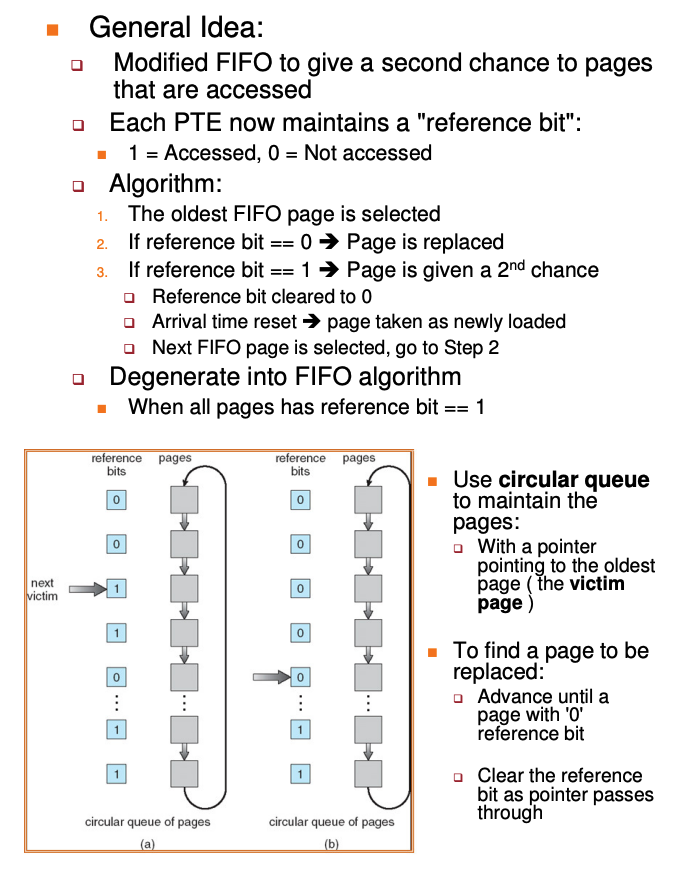
\includegraphics[width=0.24\textwidth]{page_replace_clock}
      \end{center}
  \subsection*{Frame allocation}
    \subsubsection*{Simple approaches}
      \paragraph{Equal allocation} process gets same amount of frames
      \paragraph{Proportional allocation} process gets frames proportional to memory usage
    \subsubsection*{Local/Global replacement}
      \paragraph{Local} Evicted page selected from the process
        \ull {
          \tick Thrashing limited to the process (but it can use up I/O bandwith and degrade performance of other processes)
          \cross Insufficient frames can hinder progress
        }
      \paragraph{Global} Evicted page selected from all frames
        \ull {
          \tick Process that needs more frames can get from others that need less
          \cross Can cause thrashing in other processes (cascading thrashing)
        }
    \subsubsection*{Working set model}
      \ull {
        \item Define working set $W(t, \Delta)$ as the set of active pages in the interval at time $t$
        \item Allocate sufficient frames for pages in $W(t, \Delta)$ to reduce chance of page fault
        \item Relatively constant in a period of time (locality)
        \item Too small: may miss pages in current working set
        \item Too big: may contain pages from a different working set
      }
      \begin{center}
        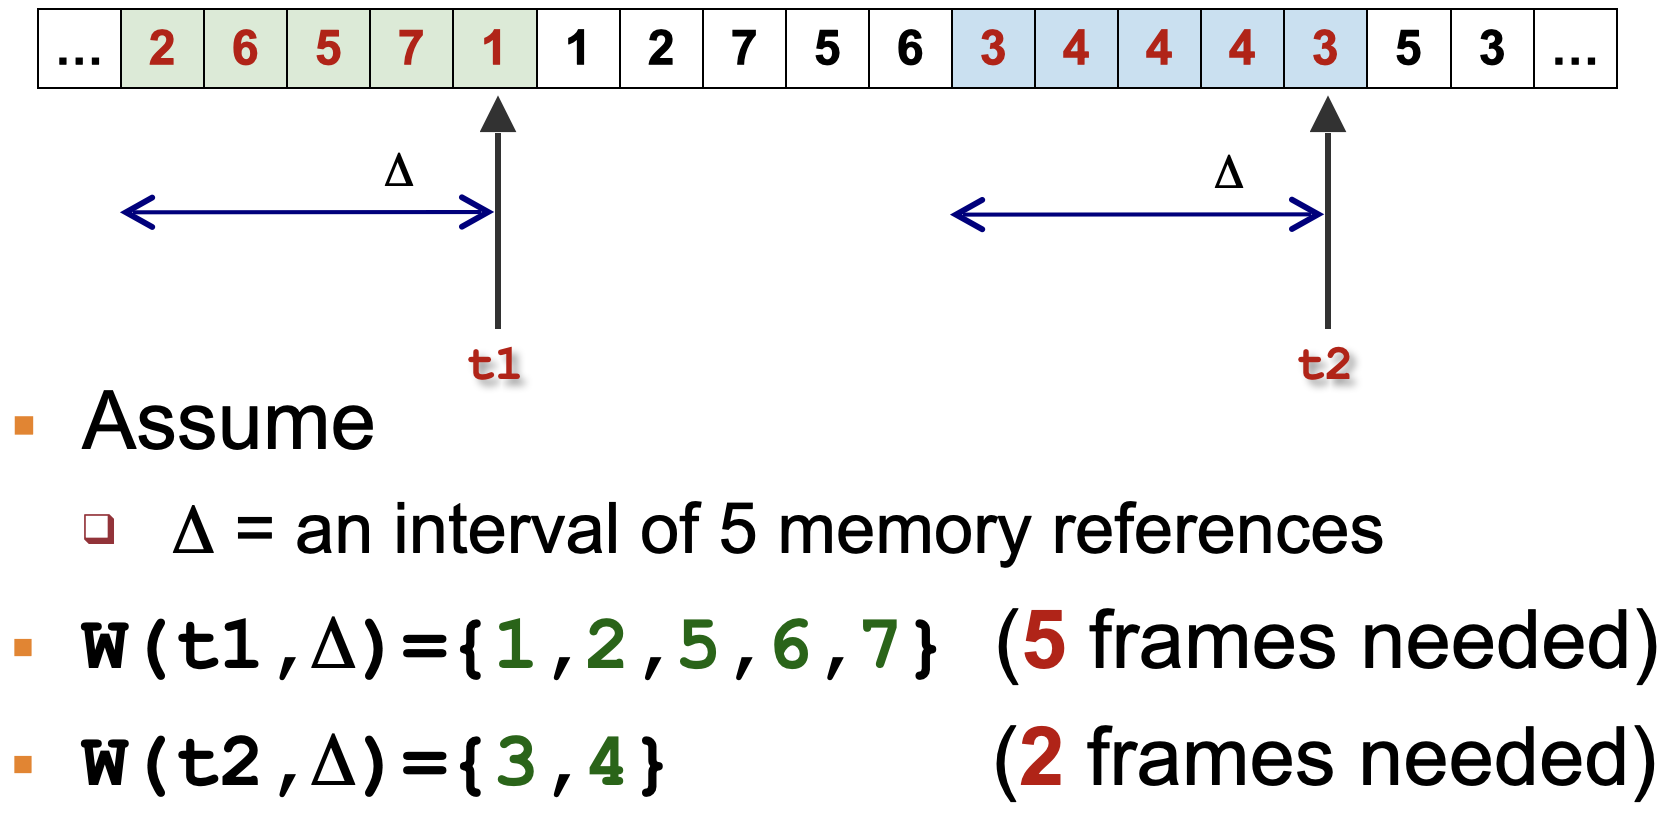
\includegraphics[width=0.24\textwidth]{working_set_model}
      \end{center}
\section*{File \kern-0.06em system \kern-0.13em management}
  \subsection*{Misc}
    \subsubsection*{Motivation}
      \ull {
        \item Physical memory is volatile (only maintains data while powered), so we want to use external storage to store persistent info
        \item Provide an abstraction over external storage
        \item Provide protection and sharing bewteen processes and users
      }
    \subsubsection*{Hard disk layout}
      \begin{center}
        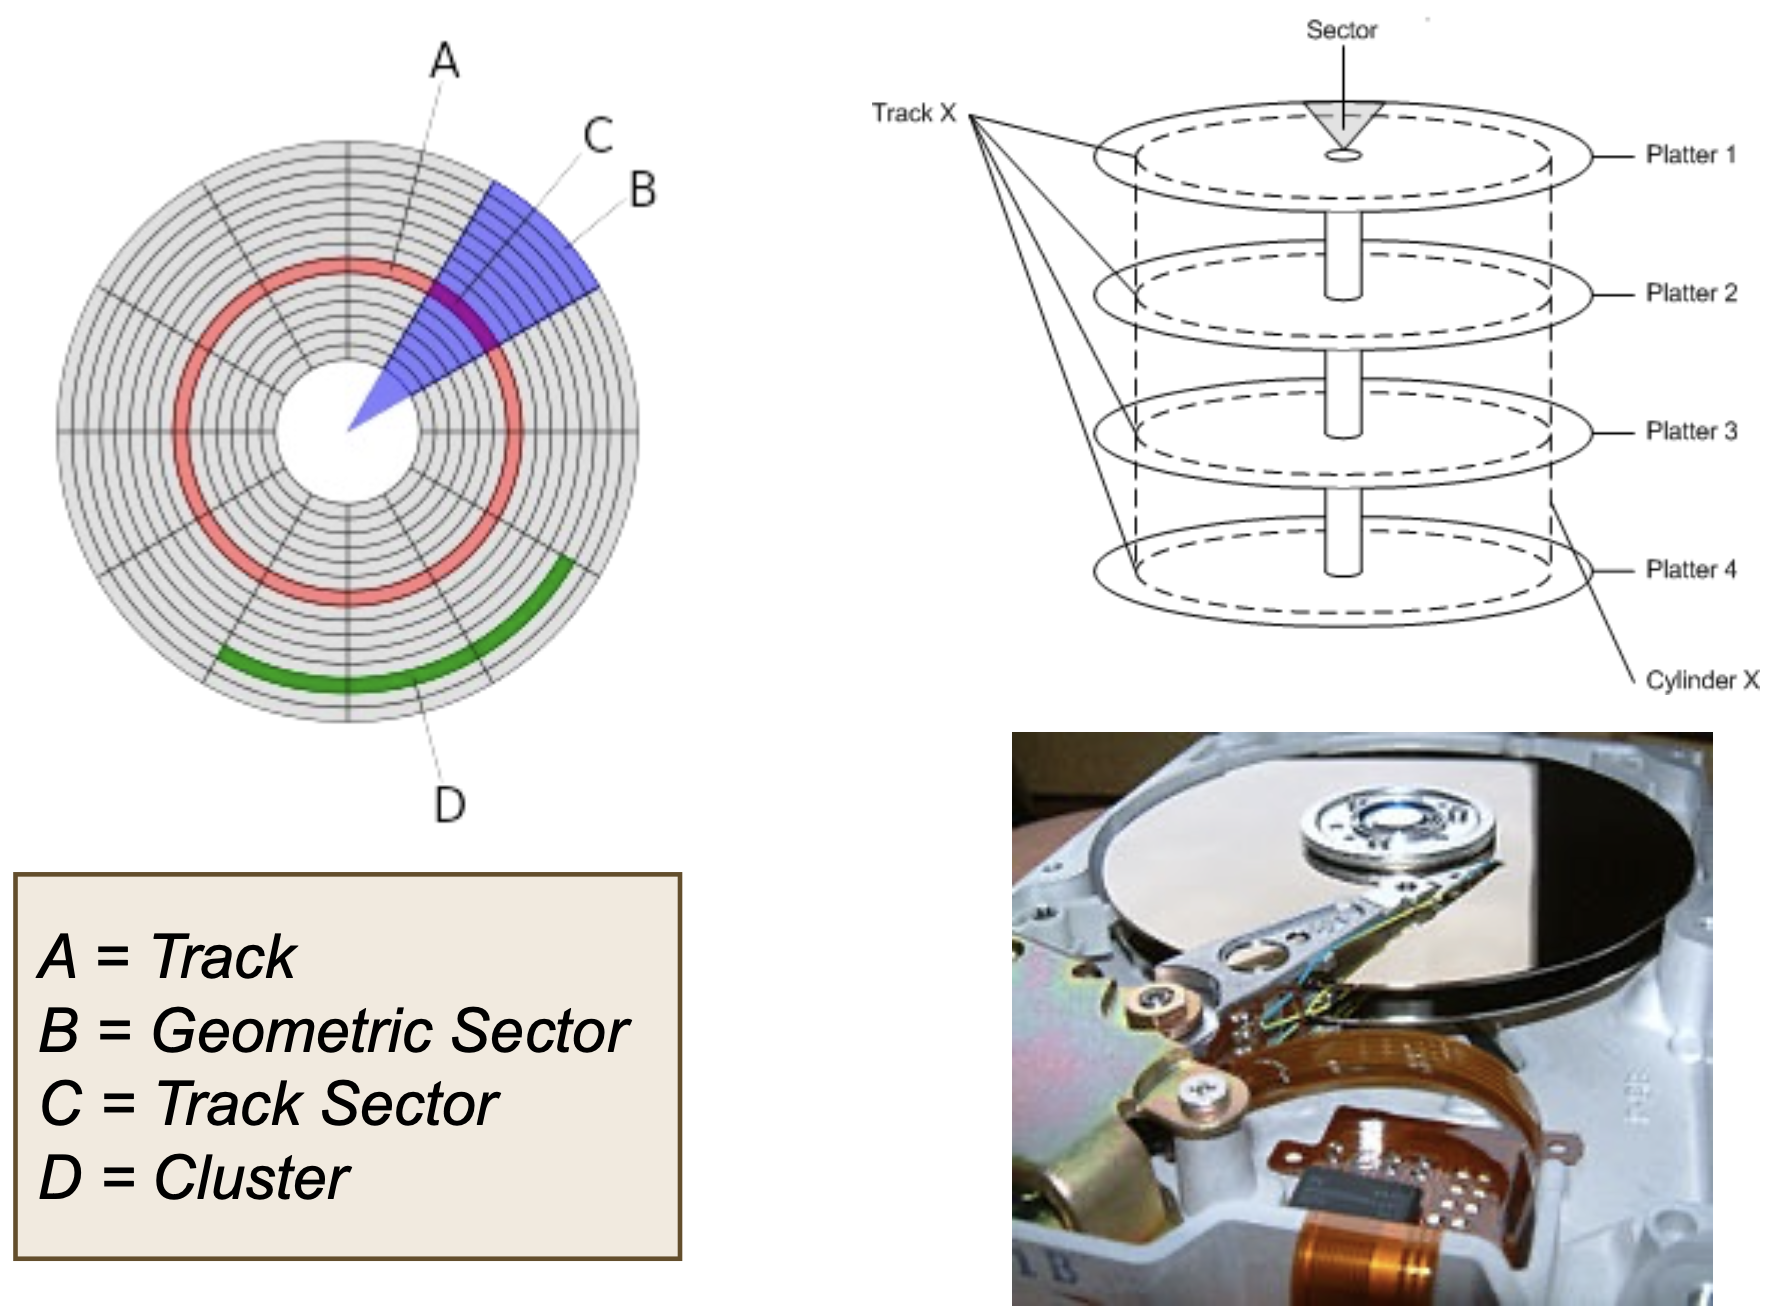
\includegraphics[width=0.24\textwidth]{hard_disk}
      \end{center}
    \subsubsection*{General criteria} \noindent
      Self-contained, Persistent, Efficient
  \subsection*{File}
    \ull {
      \item Contains data
      \item Contains metadata (name, identifier, type, size, protection, time/date/owner info, table of content)
    }
    \subsubsection*{File name} \noindent
      Different FS has different naming rules (length, case sensitivity, special symbols, extension)
    \subsubsection*{File type}
      \ull {
        \item Each file type has an associated set of operations; possibly a specific program for processing
        \item Regular files, directories, special files
      }
      \paragraph{Regular files}
        \ull {
          \item ASCII files: can be printed as is (text file, source code)
          \item Binary files: have a predefined structure to be processed by a specific program (executable, Java class file, pdf file)
        }
      \paragraph{Distinguishing file type}
        \ull {
          \item Windows uses file extension
          \item Unix uses embedded info in the file (magic number)
        }
    \subsubsection*{File size} \noindent
      Usually does not include file metadata
    \subsubsection*{File protection} \noindent
      Read, Write, Execute, Append, Delete, List (Read metadata of a file)
      \paragraph{Permission bits}
        \ull {
          \item Classify users into Owner/Group/Universe
          \item Unix stores RWX for each of the 3 classes of users
        }
      \paragraph{Tut 10/11 DirExp} \noindent \\
        Think of directory as the list of directory entries
        \ull {
          \item Read = Can you read this list (ls, tab auto-completion)
          \item Write = Can you change this list (create, rename, delete entry)
          \item Execute = Can you use this directory as WD (cd)
        }
        \begin{center}
          \begin{tabular}{ |c|c|c|c| }
            \hline
            Action & \ic{r-x} & \ic{-wx} & \ic{--x} \\ \hline
            \ic{ls -l DIR} & ok & no & no \\ \hline
            \ic{cd DIR} & ok & ok & ok \\ \hline
            \multicolumn{4}{|c|}{After \ic{cd}} \\ \hline
            \ic{ls -l} & ok & no & no \\ \hline
            \ic{cat curfile} & ok & ok & ok \\ \hline
            \ic{touch curfile} & ok & ok & ok \\ \hline
            \ic{touch newfile} & nope & ok & nope \\ \hline
          \end{tabular}
        \end{center}
    \subsubsection*{File metadata} \noindent
      Rename, Change attributes, Read attributes
    \subsubsection*{File data} \noindent
      \ull {
        \item Array of bytes
        \item Fixed length records (can jump to any record easily)
        \item Variable length records (flexible but harder to locate a record)
      }
      \paragraph{Records}
        \ull {
          \item In C files, each record is a character
          \item In a SQL database, each record is a row in the table, and it could be fixed length if there are no variable length string attributes
          \item In video files, each record is a compressed frame (simplified), which has variable length, depending on the compression rate of the individual frames
        }
      \paragraph{Access methods}
        \ull {
          \item Sequential: read in order
          \item Random: read in any order
            \ull {
              \item \ic{Read(Offset)}: explicitly state position to access
              \item \ic{Seek(Offset)}: special op to move to a new location in file
            }
          \item Direct: allow random access to any record
        }
      \paragraph{Generic operations} \noindent
        Create, Open, Read, Write, Repositioning (Seek), Truncate
  \subsection*{File operations} \noindent
    OS provides file ops as syscalls:
    \ull {
      \item Provide protection, concurrent and efficient access
      \item Maintain info
    }
    \subsubsection*{Info to keep for an opened file} \noindent
      File pointer, Disk location, Open count (how many processes has this file opened)
    \subsubsection*{Open-file table}
      \ull {
        \item System-wide file table: one entry per unique file
        \item Process file table: one entry per file used in process, each entry points to the system-wide table
      }
      \begin{center}
        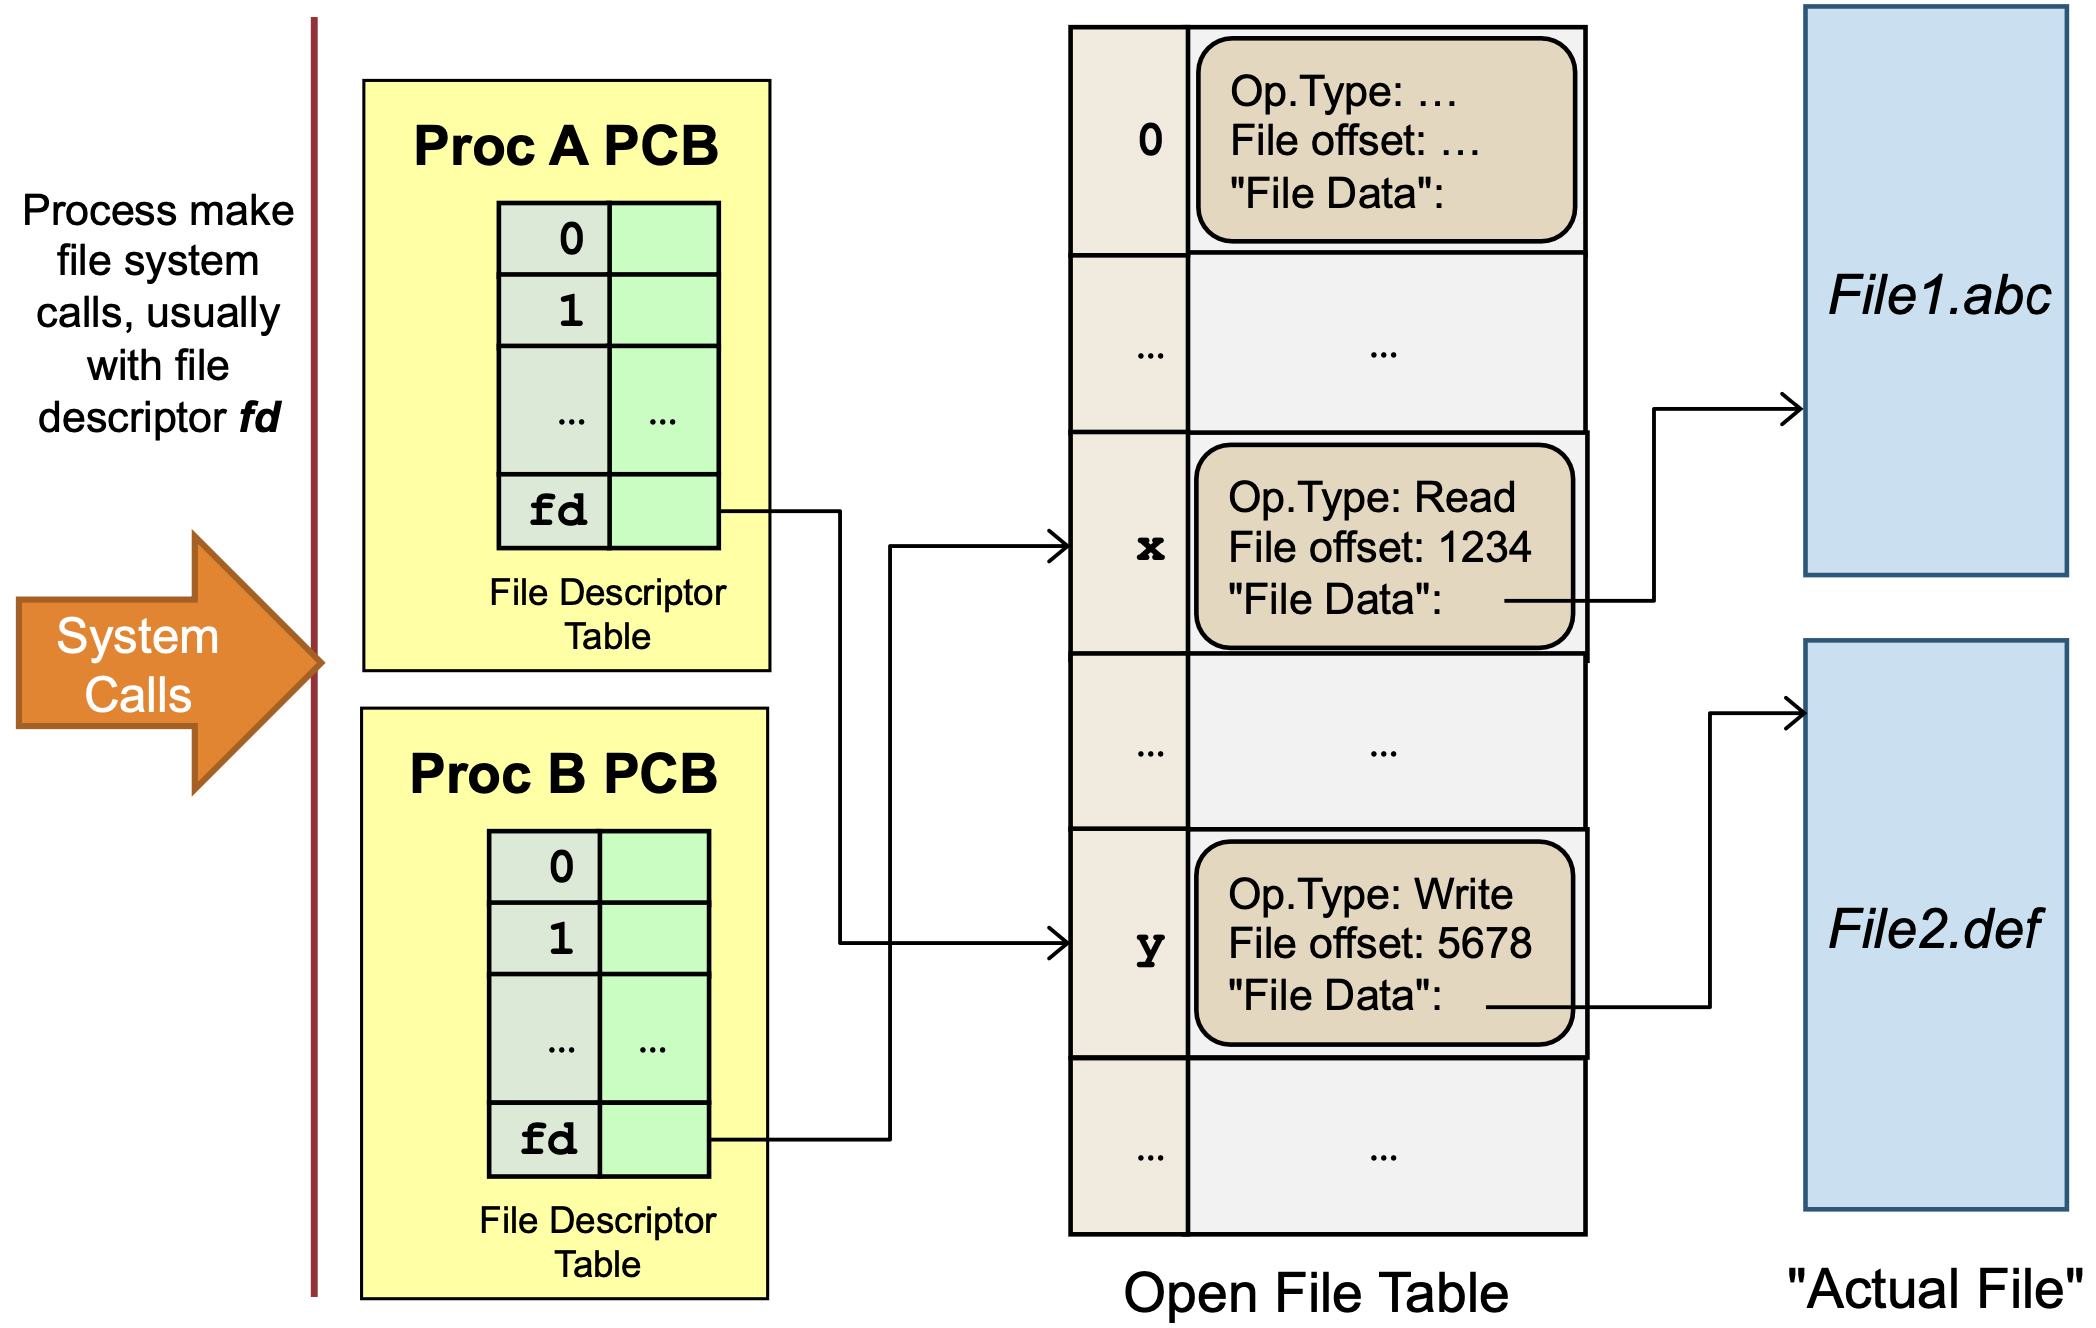
\includegraphics[width=0.24\textwidth]{open_file_table}
      \end{center}
      \paragraph{Process sharing}
        \ull {
          \item Two processes with different FDs pointing to the same file can do I/O independently
          \item \ic{fork()}: Two processes with the same FD will share 1 FD
        }
  \subsection*{Directory}
    \subsubsection*{Purpose} \noindent
      Provide a logical grouping of files, Keep track of files
    \subsubsection*{Structure} \noindent
      Single-level, Tree, DAG, General graph
    \subsubsection*{Links}
      \paragraph{Hard link}
        \ull {
          \item Maintain separate pointers to the same file
          \item Only for files, creates DAG
        }
      \paragraph{Soft link}
        \ull {
          \item A file that contains the path name of the file to link to (essentially like a shortcut)
          \item Files and directories, creates general graph
        }
      \paragraph{Unix symbolic link (soft link)} Symlinks always have permissions 777 (so anyone may use the symlink), but the actual access permissions are checked against the original file linked to
\section*{File system\\implementations}
  \subsection*{Generic disk organization} \noindent
    Note: MBR is Master Boot Record
    \begin{center}
      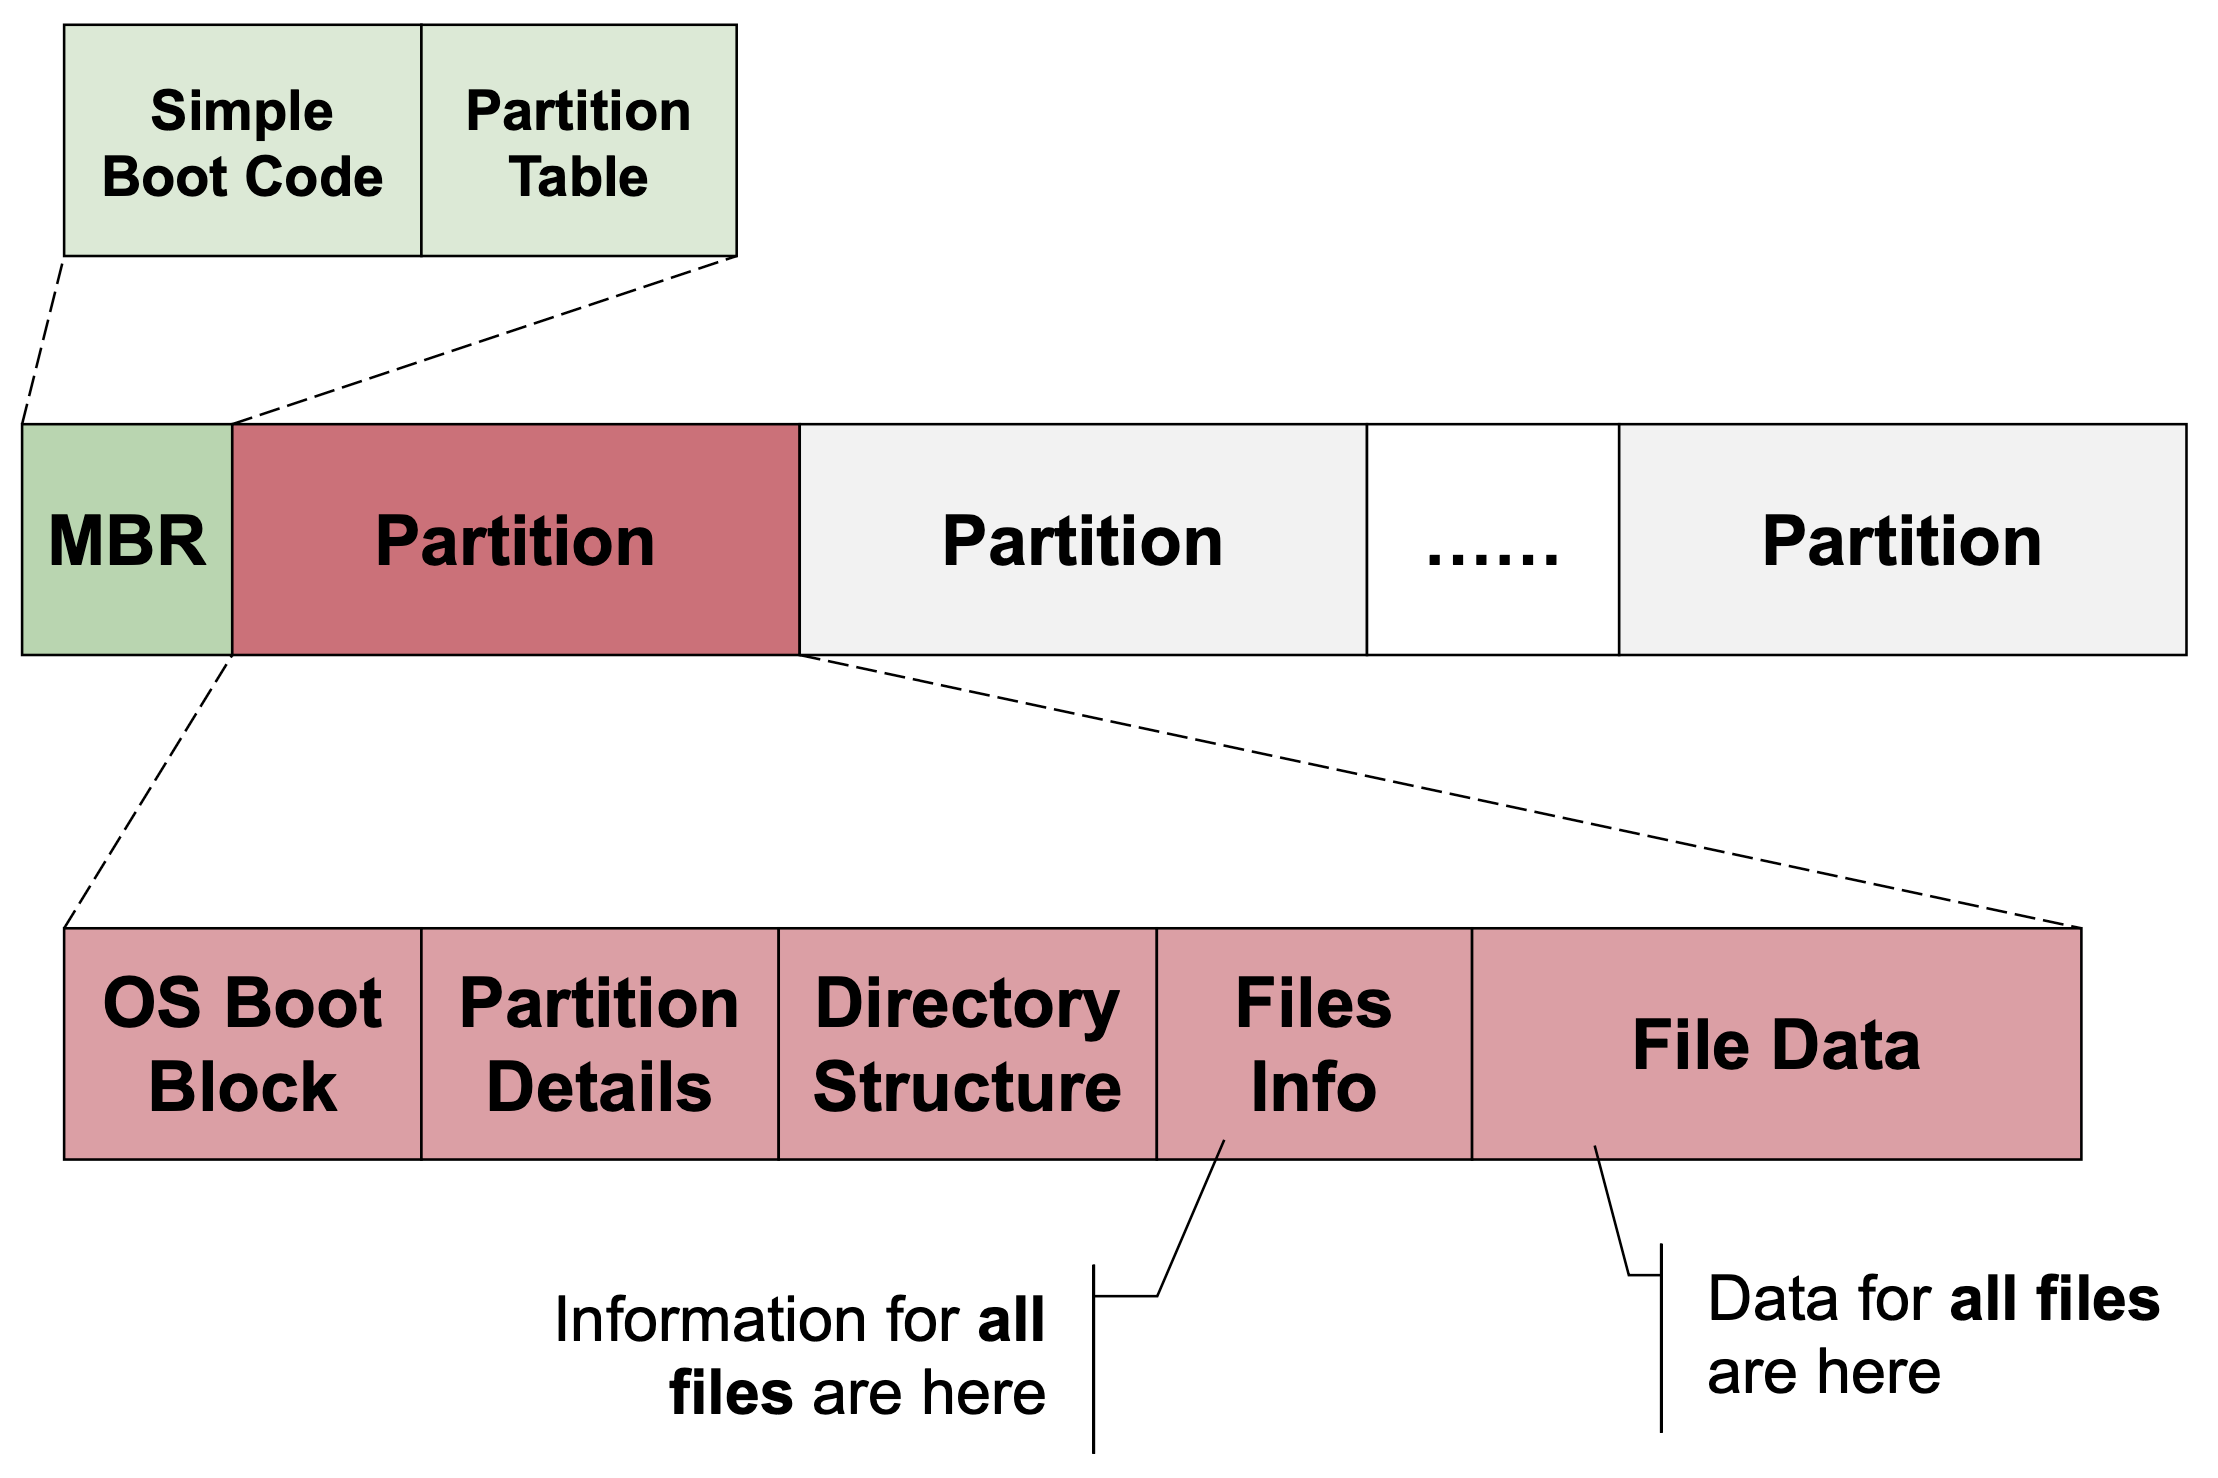
\includegraphics[width=0.24\textwidth]{generic_disk_organization}
    \end{center}
  \subsection*{File block allocation} \noindent
    Note: all can have internal fragmentation, if the last block is not full (at least by CS2106 definitions)
    \subsubsection*{Contiguous}
      \ull {
        \item Allocate consecutive disk blocks to a file
        \item Each file stores start block and length
        \tick Simple to keep track
        \tick Fast access (only need to seek to first block)
        \cross External fragmentation
        \cross File size needs to be specified in advance
      }
    \subsubsection*{Linked list}
      \ull {
        \item Each disk block additionally stores next disk block number (i.e. pointer)
        \item Each file stores first block and last block
        \tick No external fragmentation
        \cross Random access in a file is very slow
        \cross Part of disk block is used for pointer
        \cross Less reliable (if one of the pointers is incorrect, you might lose the rest of the data)
      }
    \subsubsection*{File Allocation Table (FAT)}
      \ull {
        \item Linked list v2.0
        \item Store all disk block pointers in a single table (FAT), which is in memory all the time
        \tick Faster random access (than linked list)
        \cross Keeps track of all disk blocks in a partition (can be huge, consumes valuable memory space)
      }
    \subsubsection*{Indexed}
      \ull {
        \item Each file has an index block, an array of disk block addresses of the disks that contain the file data
        \tick Lesser memory overhead than FAT (only index block of opened file needs to be in memory)
        \tick Fast direct access
        \cross Limited max file size (limited to block size)
        \cross Index block overhead
      }
    \subsubsection*{Indexed + linked list}
      \ull {
        \item Keep a linked list of index blocks
        \item Each index block contains the pointer to the next index block
      }
    \subsubsection*{Multilevel indexing}
      \ull {
        \item Like multilevel paging but for blocks
        \item Can be generalized to any number of levels, but if a scheme is decided, then there is a limit to the file size
      }
    \subsubsection*{Unix I-node} \noindent
      12 direct pointers, 1 single indirect block, 1 double indirect block, 1 triple indirect block
      \begin{center}
        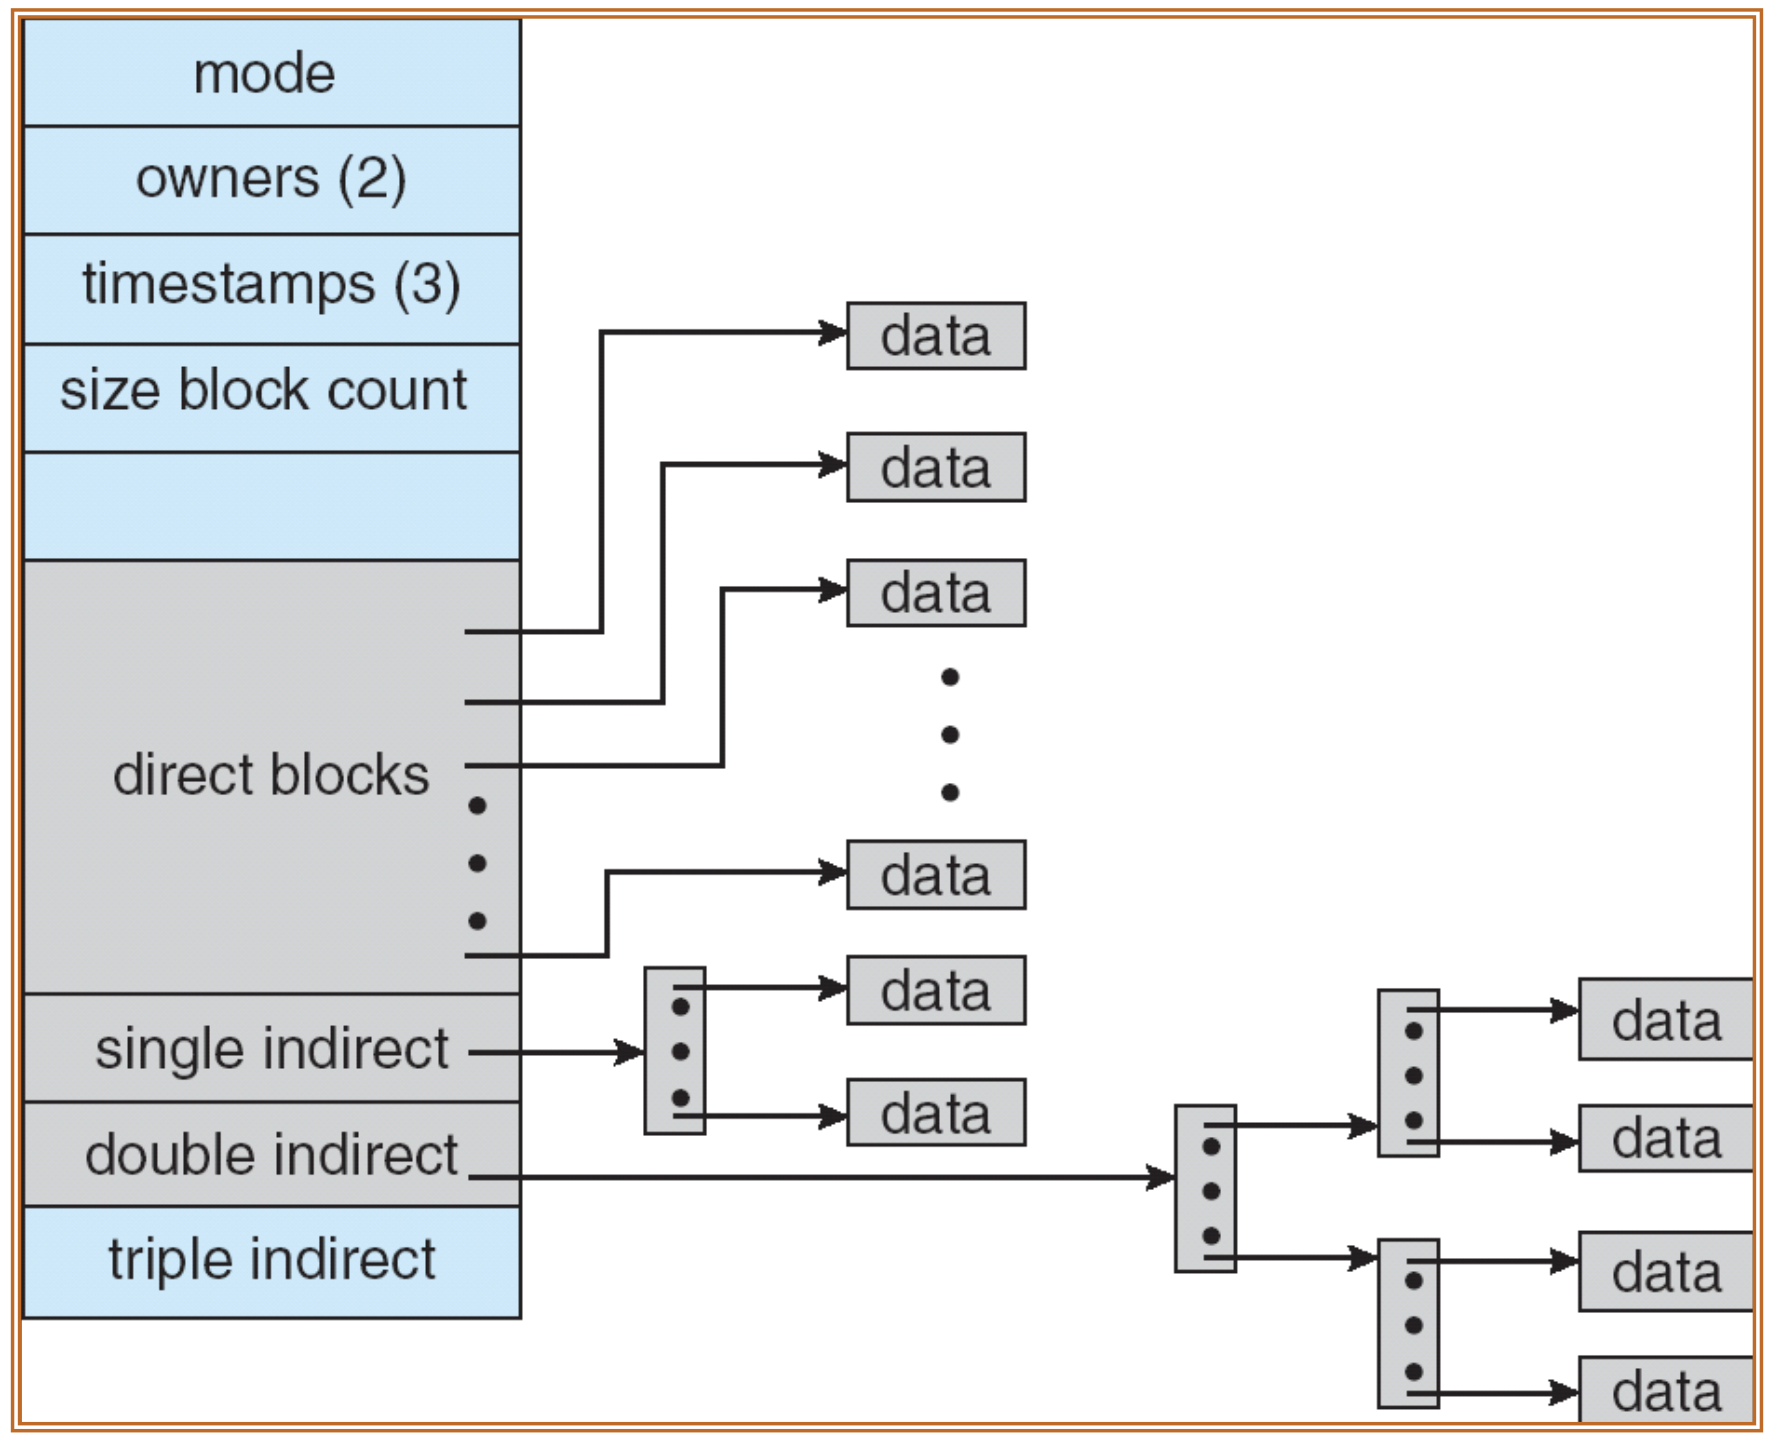
\includegraphics[width=0.24\textwidth]{unix_inode}
      \end{center}
  \subsection*{Free space management} \noindent
    To manage free disk blocks
    \subsubsection*{Bitmap}
      \ull {
        \item Each disk block is represented by 1 bit
        \item e.g. 1=free, 0=occupied
        \tick Powerful bit manipulations
        \cross Need to keep the bitap in memory for efficiency reasons
      }
    \subsubsection*{Linked list}
      \ull {
        \item Linked list of disk blocks
        \item Each node (disk block) contains some free disk block numbers, and a pointer to the next free space disk block
        \tick Easy to find free block
        \tick Only need the first pointer in memory (can cache the other blocks for efficiency)
        \cross High overhead (can be mitigated by storing the free block list in free blocks)
      }
  \subsection*{Directory}
    \subsubsection*{Traversal}
      \ull {
        \item Given a full path name
        \item Recursively check existence of each directory along the path to arrive at file info
        \item Stop if not found (or incorrect type)
      }
    \subsubsection*{Linked list}
      \ull {
        \item Each entry represents a file (file name, pointer to file info / actual file info)
        \cross Locating a file requires linear search (but can cache searches)
      }
    \subsubsection*{Hash table}
      \ull {
        \item Each directory has a hash table of size N
        \item Hash file name to locate file
        \item Usually use hash table with chaining
        \tick Fast lookup
        \cross Hash table has limited size
        \cross Depends on good hash function
      }
    \subsubsection*{File information} \noindent
      Consists of file name, metadata, disk block info
      \oll {
        \item Store everything in directory entry, or
        \item Store file name and point to another DS for other info
      }
  \subsection*{Disk scheduling}
    \begin{center}
      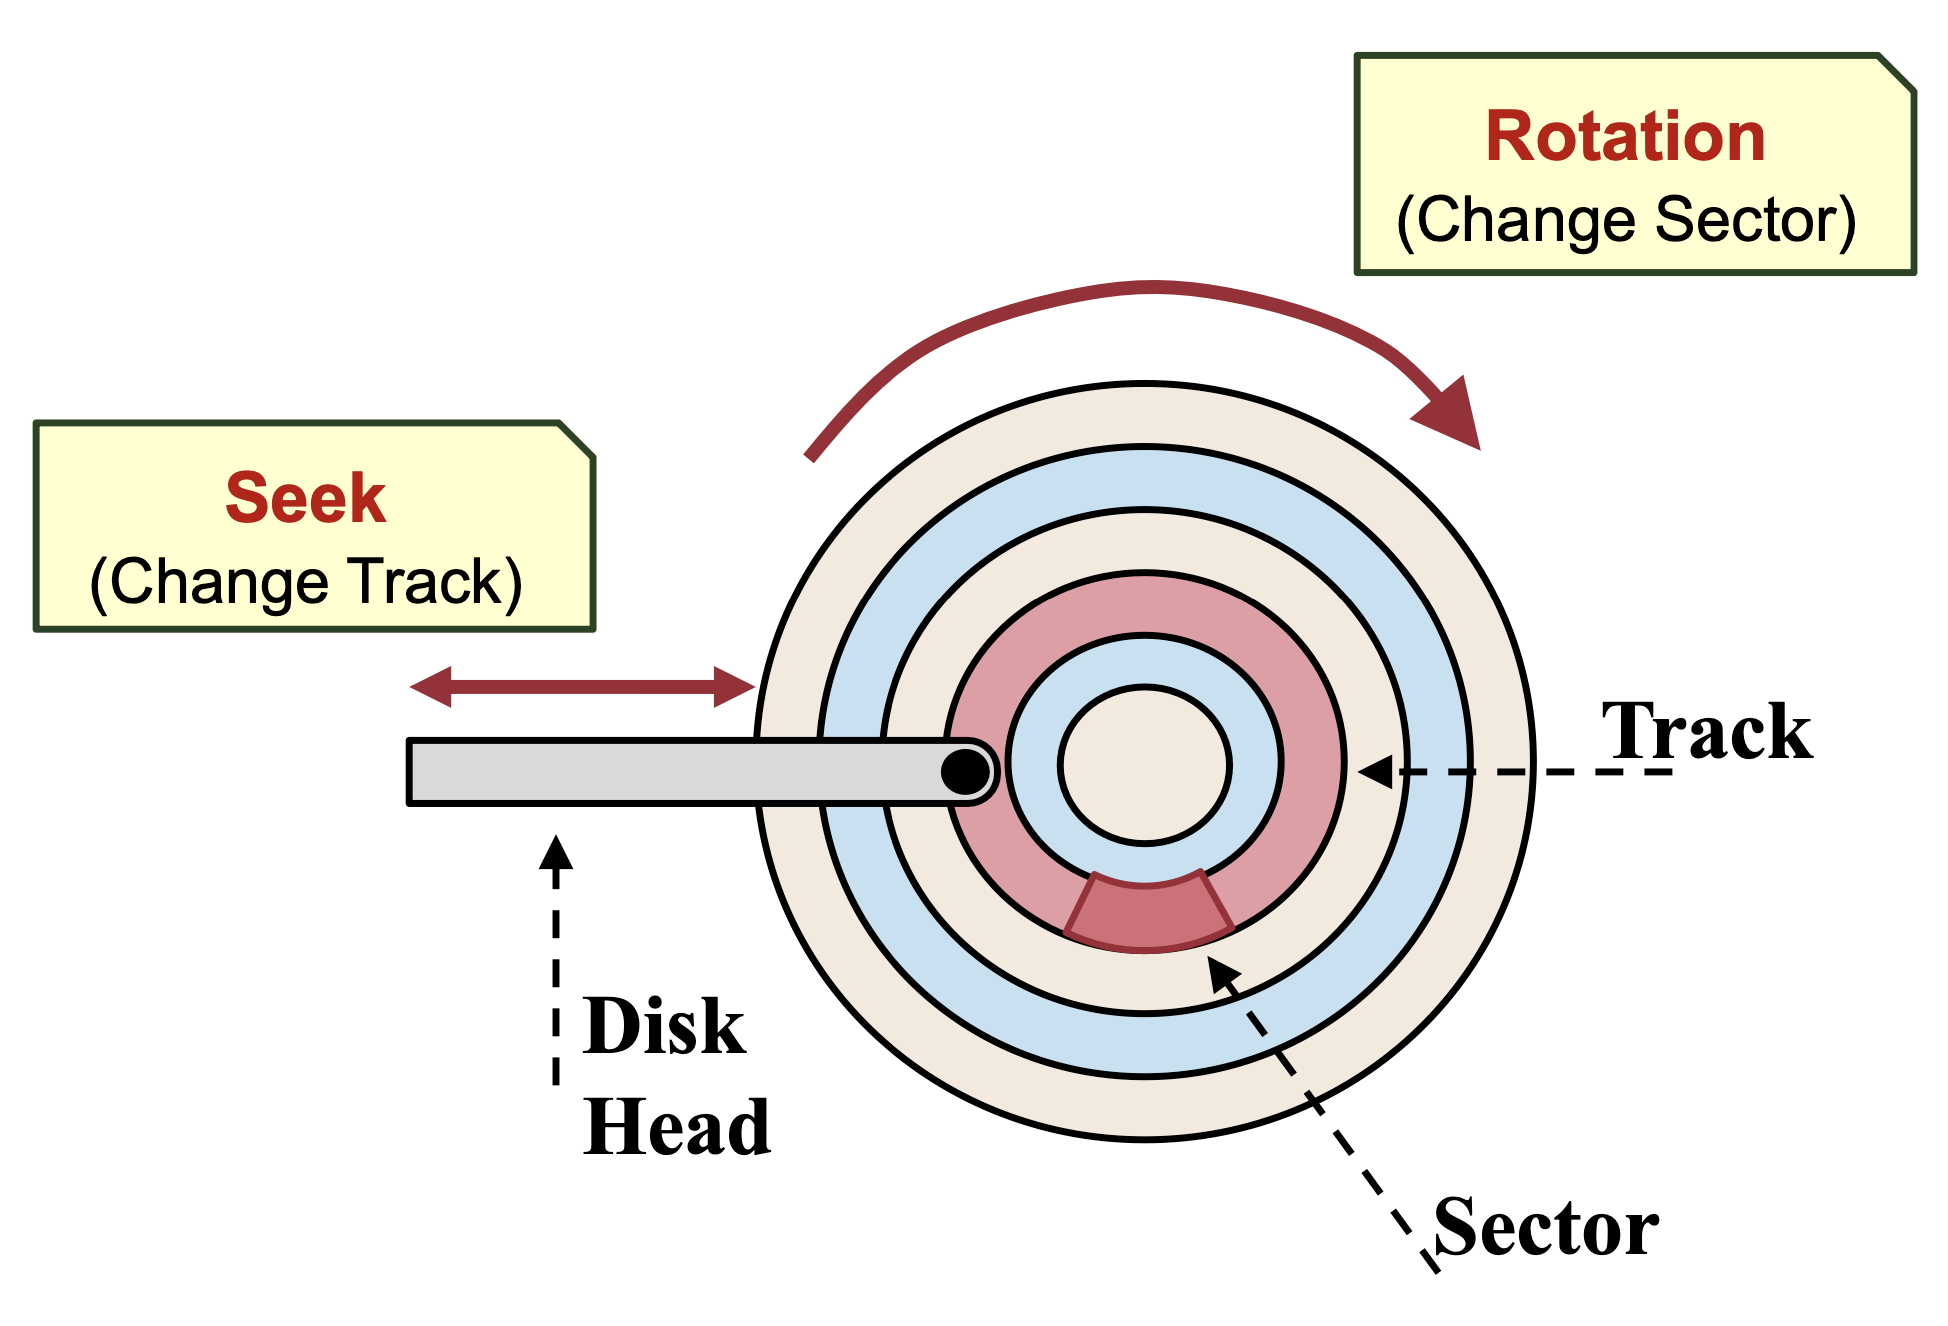
\includegraphics[width=0.24\textwidth]{magnetic_disk}
    \end{center}
    \subsubsection*{I/O latency}
      \oll {
        \item Position disk head over proper track (Seek time)
          \ull {
            \item Position the disk head over the proper track
            \item Average typically around 2ms to 10ms
            \item Expected seek time is $T/3$ where $T$ is the time for max seek distance
          }
        \item Wait for desired sector to rotate under the read/write head (Rotational latency)
          \ull {
            \item 4800 to 15000 RPM (12.5ms to 4ms per rotation)
            \item Assume desired data is halfway around track, then average rotational latency is 6.25ms at 4800RPM, 2ms at 15000RPM
          }
        \item Transfer the sector(s) from disk to memory (Transfer time)
          \begin{center}
            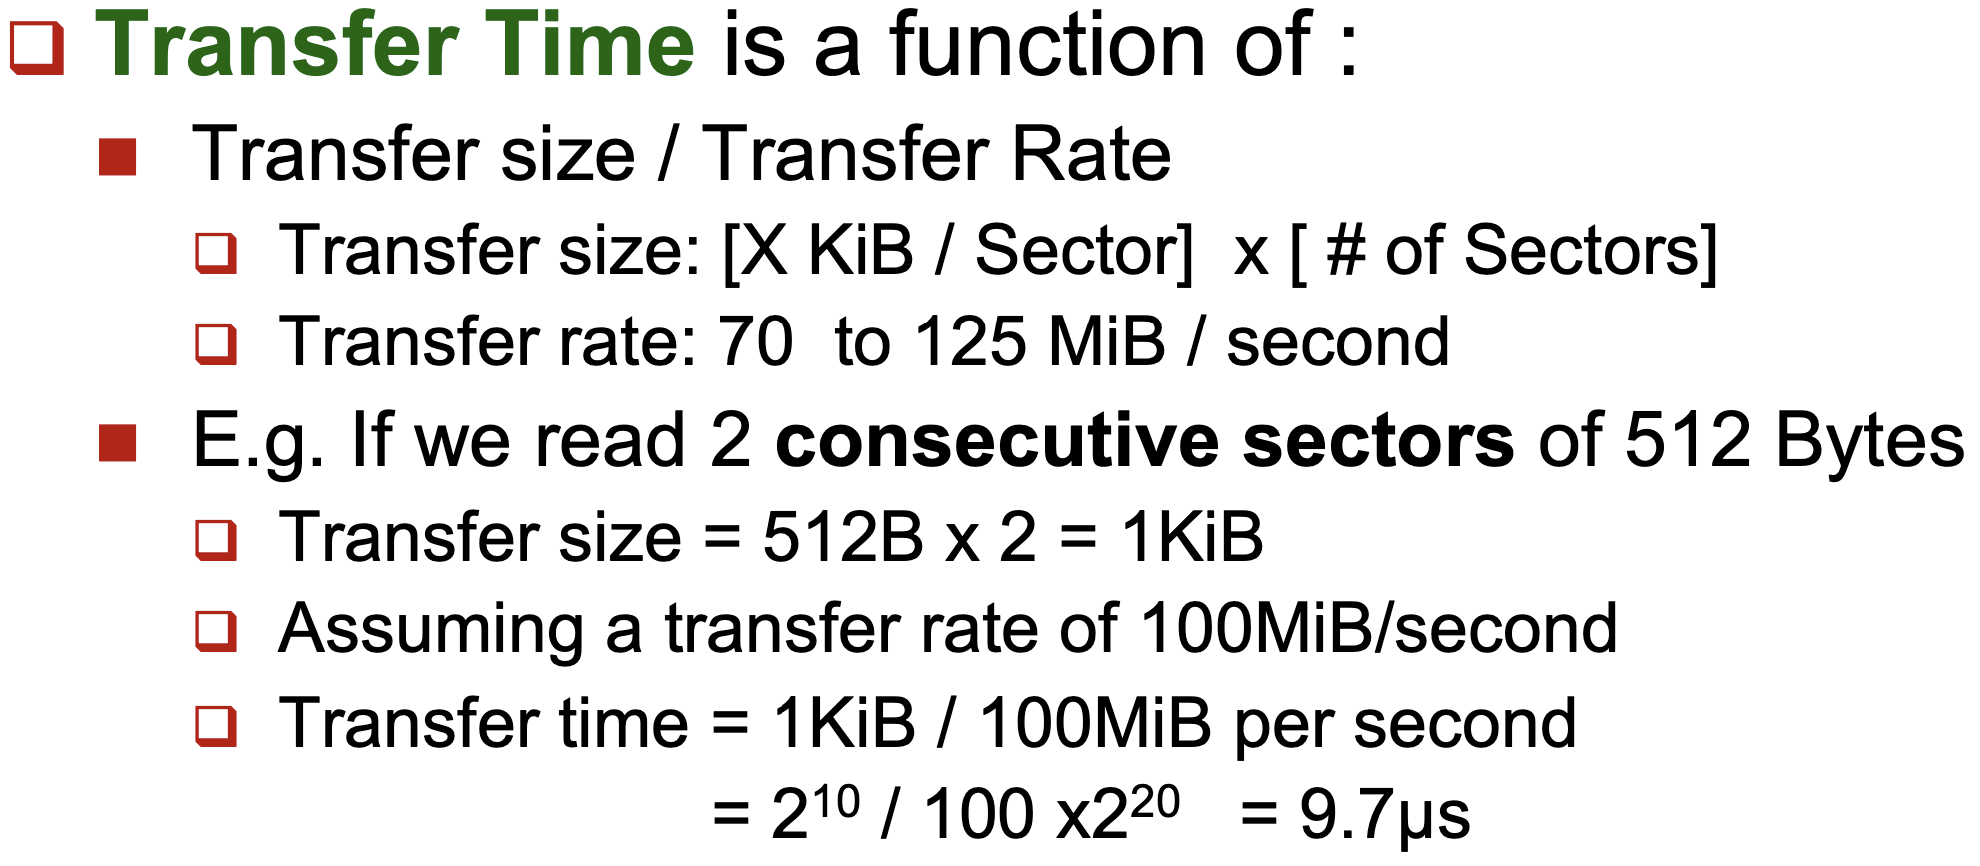
\includegraphics[width=0.22\textwidth]{transfer_time}
          \end{center}
          \ull {
            \item (1) and (2) are 3 orders of magnitude slower than (3)
          }
      }
  \subsubsection*{Disk scheduling algorithms}
    \ull {
      \item First come first serve
      \item Shortest seek first
      \item SCAN (elevator)
      \item C-SCAN (outside to inside and repeat)
    }
\section*{File system\\case studies}
  \subsection*{FAT}
    \subsubsection*{Layout}
      \begin{center}
        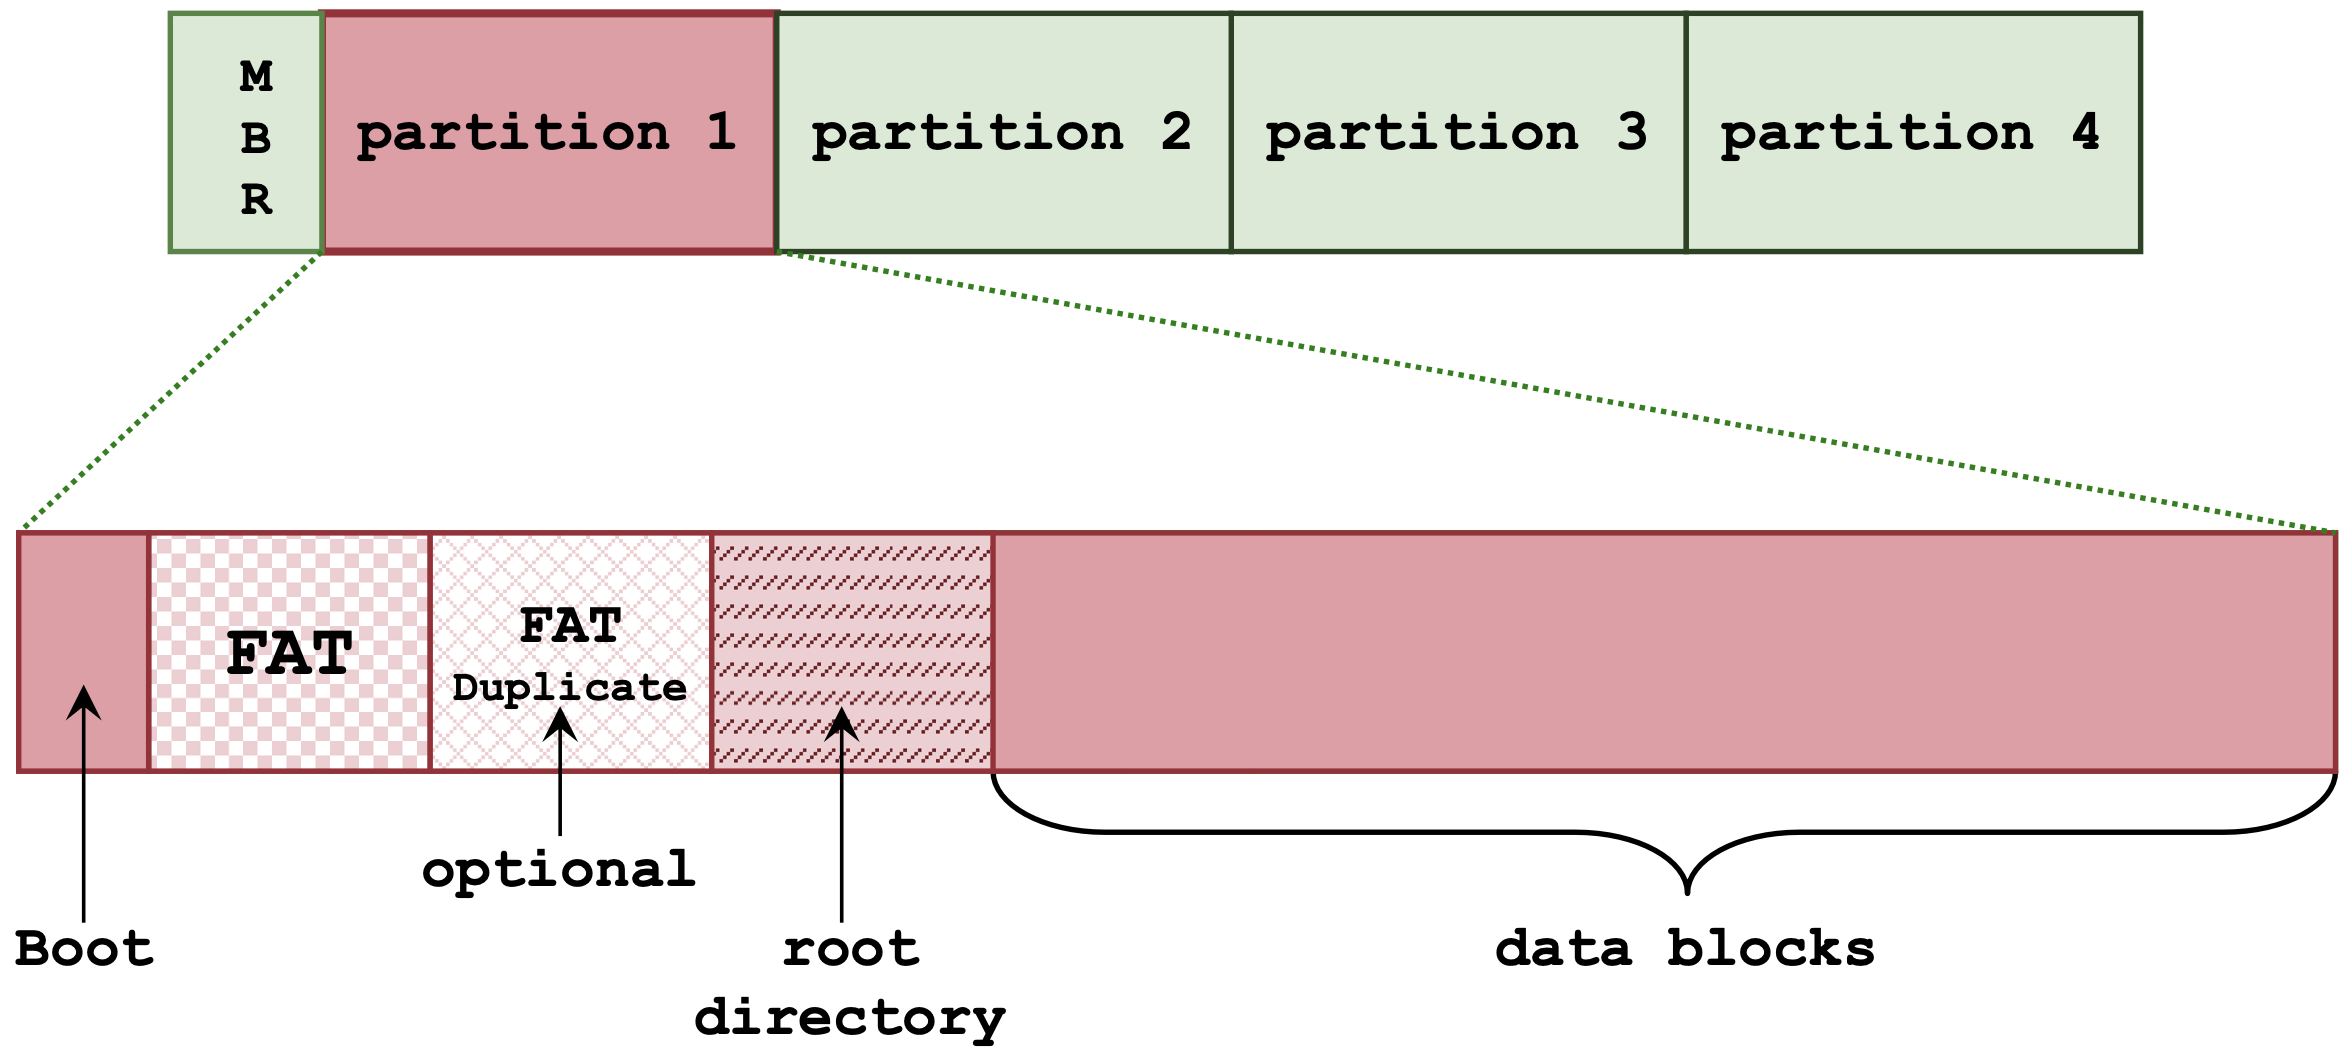
\includegraphics[width=0.24\textwidth]{FAT/layout}
      \end{center}
    \subsubsection*{FAT entry}
      \ull {
        \item FREE code (unused block)
        \item Block number of next block
        \item EOF code (i.e. NULL pointer)
        \item BAD block (block is unusable, i.e. disk error)
      }
    \subsubsection*{Directory}
      \ull {
        \item Represented as special type of file
        \item Root directory is stored in a special location, while other directories are stored in the data blocks
        \item Each file/subdirectory in the folder is represented as a directory entry
      }
    \subsubsection*{Directory entry}
      \begin{center}
        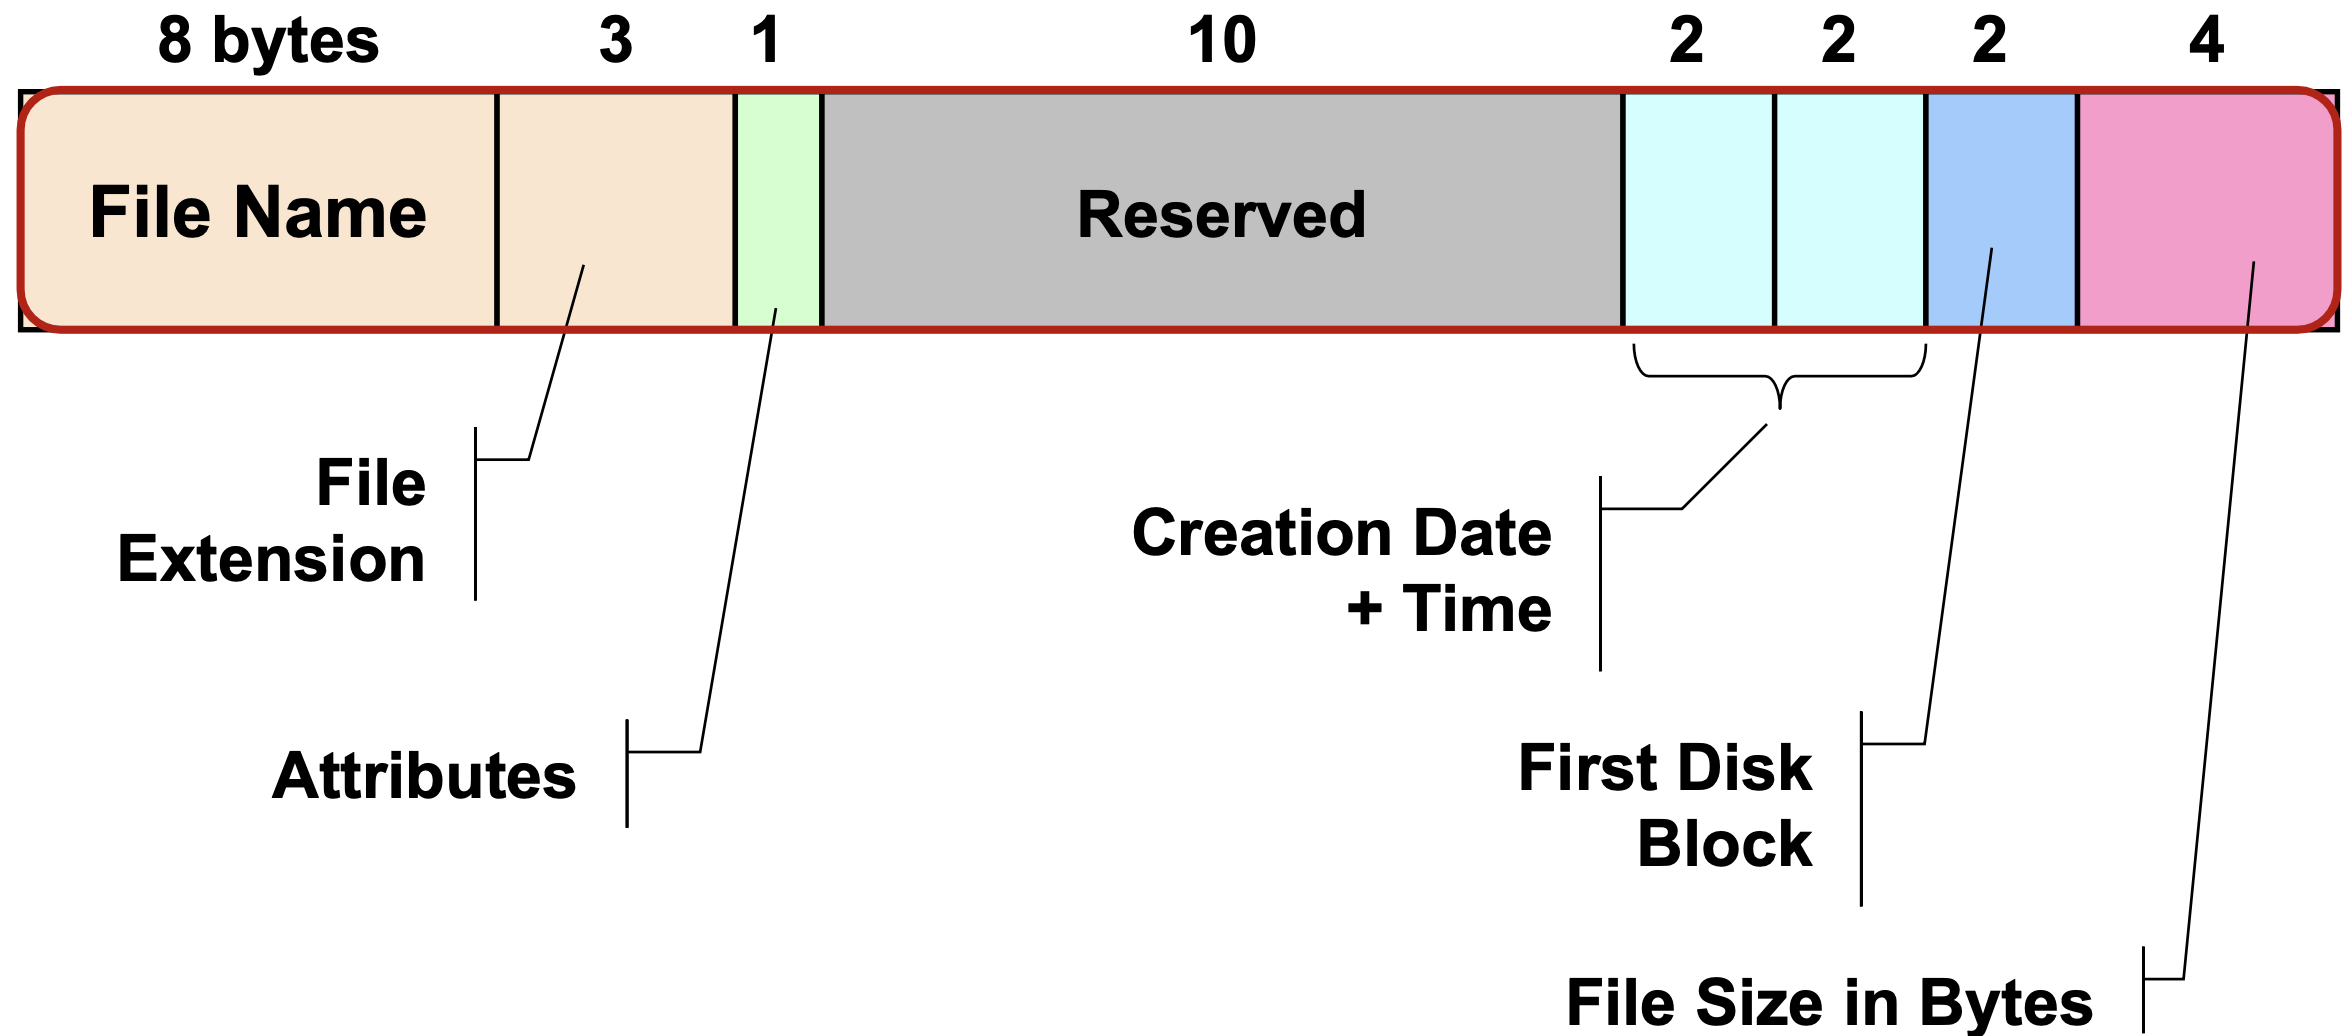
\includegraphics[width=0.24\textwidth]{FAT/directory_entry}
      \end{center}
      \ull {
        \item Fixed size - 32 bits per entry
        \item Attributes - Read-Only, Directory/File flag, Hidden, etc.
        \item First byte of file name may have special meaning (Deleted, End of directory entries, Parent directory, etc.)
        \item Creation time and date - Year limited to 1980 to 2107, accuracy of second is $\pm 2$ seconds
        \item First disk block index - 12, 16, 32 bits for FAT12, FAT16, FAT32 respectively
      }
    \subsubsection*{File deletion}
      \ull {
        \item Set first letter in filename to \ic{0xE5}
        \item Set FAT entries in linked list to FREE
        \item Can recover files as actual data blocks are intact
      }
    \paragraph{\uline{Free space management}} Must be calculuated by going through FAT
  \subsection*{FAT Variants}
    \subsubsection*{Disk cluster} \noindent
      Instead of using a single disk block as the smallest allocation unit, use a number of contiguous disk blocks
    \subsubsection*{FAT size}
      \ull {
        \item Bigger FAT $\Rightarrow$ more disk blocks/clusters $\Rightarrow$ more bits to represent each disk block/cluster (e.g. FAT12, FAT16, FAT32)
        \tick Larger cluster size $\Rightarrow$ larger usable partition
        \cross Larger cluster size $\Rightarrow$ larger internal fragmentation
        \cross FAT32: Only 28 out of 32 bits is used in disk block/cluster index (4 bits reserved)
      }
      \begin{center}
        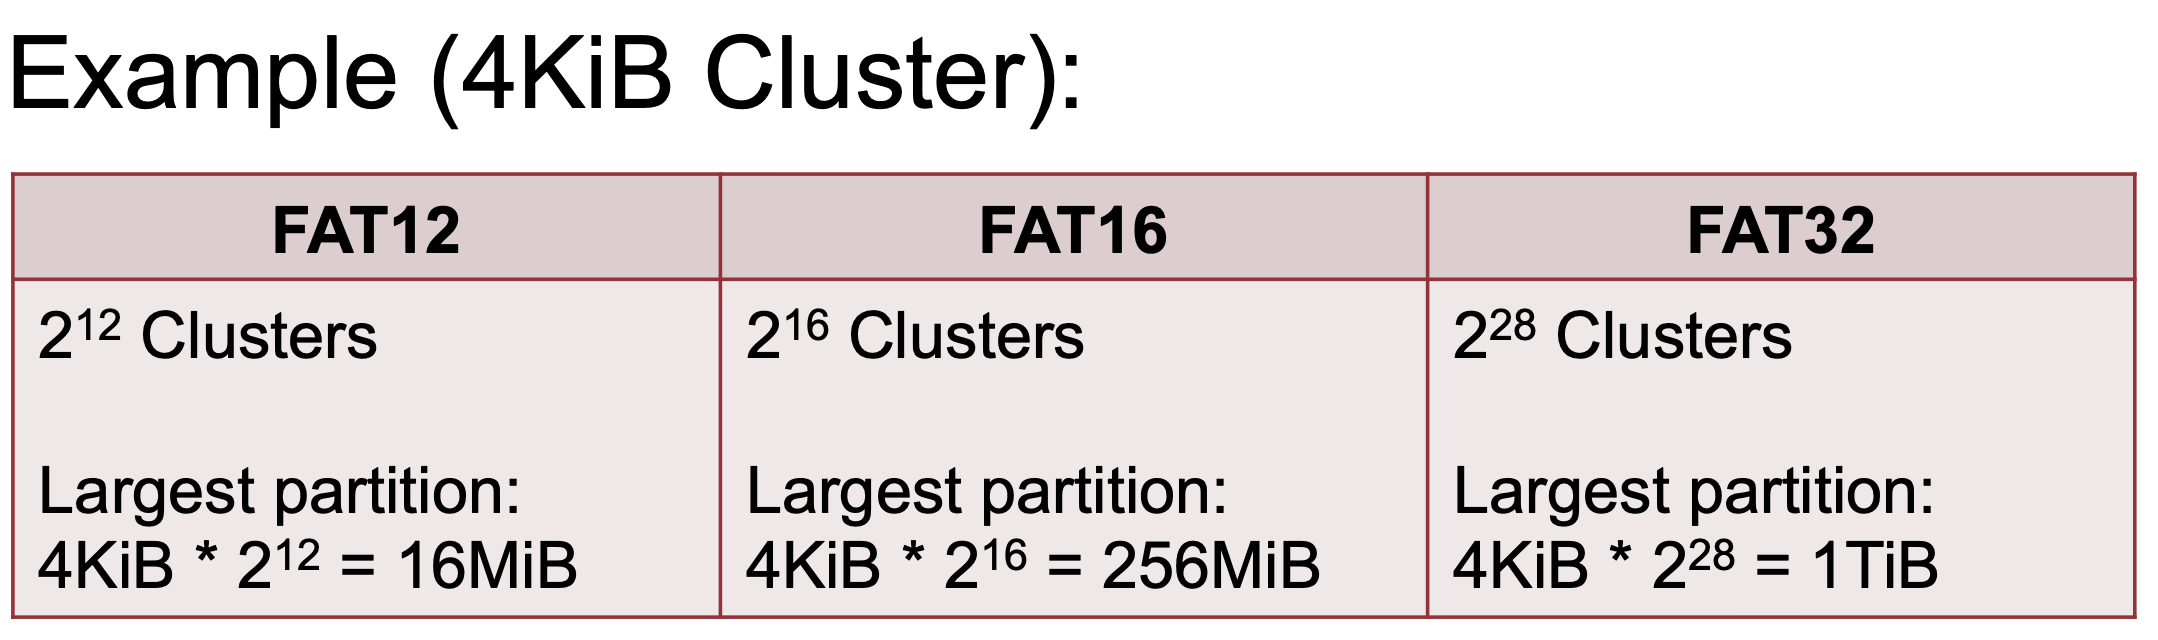
\includegraphics[width=0.24\textwidth]{FAT/cluster_size}
      \end{center}
    \subsubsection*{VFAT}
      \ull {
        \item Supports longer filenames (up to 255 chars)
        \item Workaround, uses multiple directories for a file with long name
        \item Uses invalid file attribute (so non-VFAT apps can ignore the entries)
        \item Uses first byte to indicate sequence
      }
      \begin{center}
        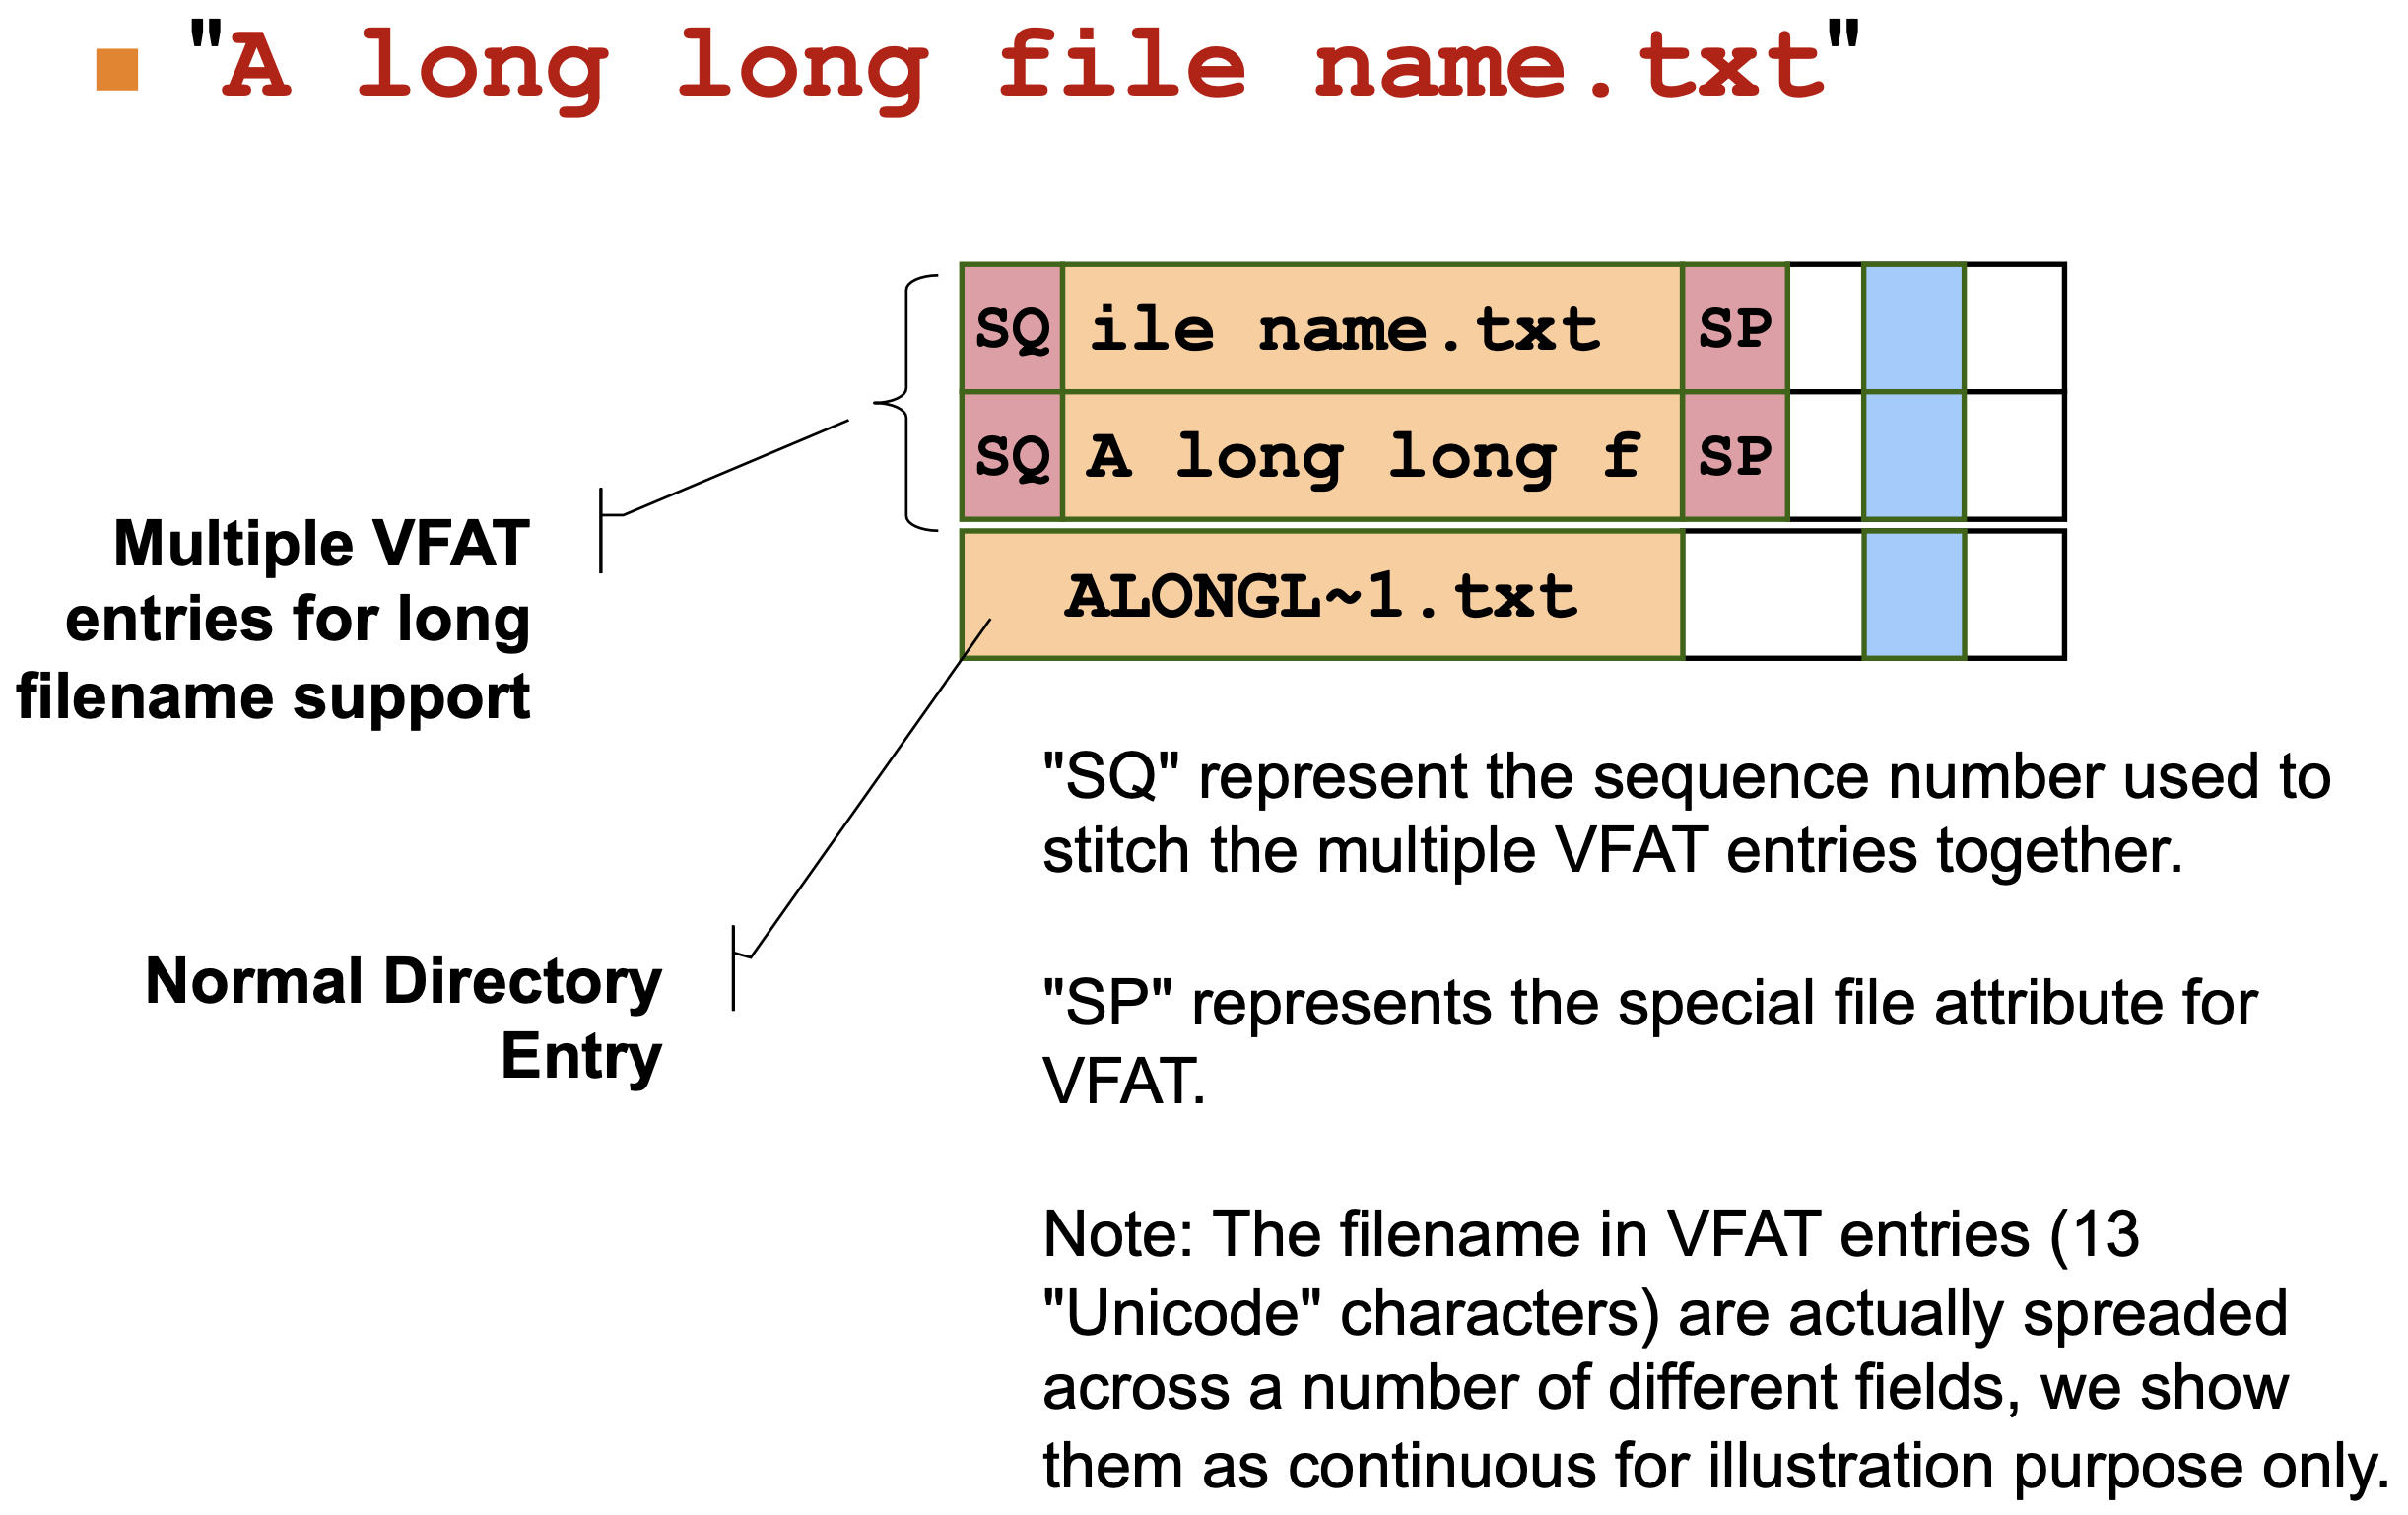
\includegraphics[width=0.24\textwidth]{FAT/vfat_entries}
      \end{center}
  \subsection*{Ext2}
    \subsubsection*{Layout}
      \begin{center}
        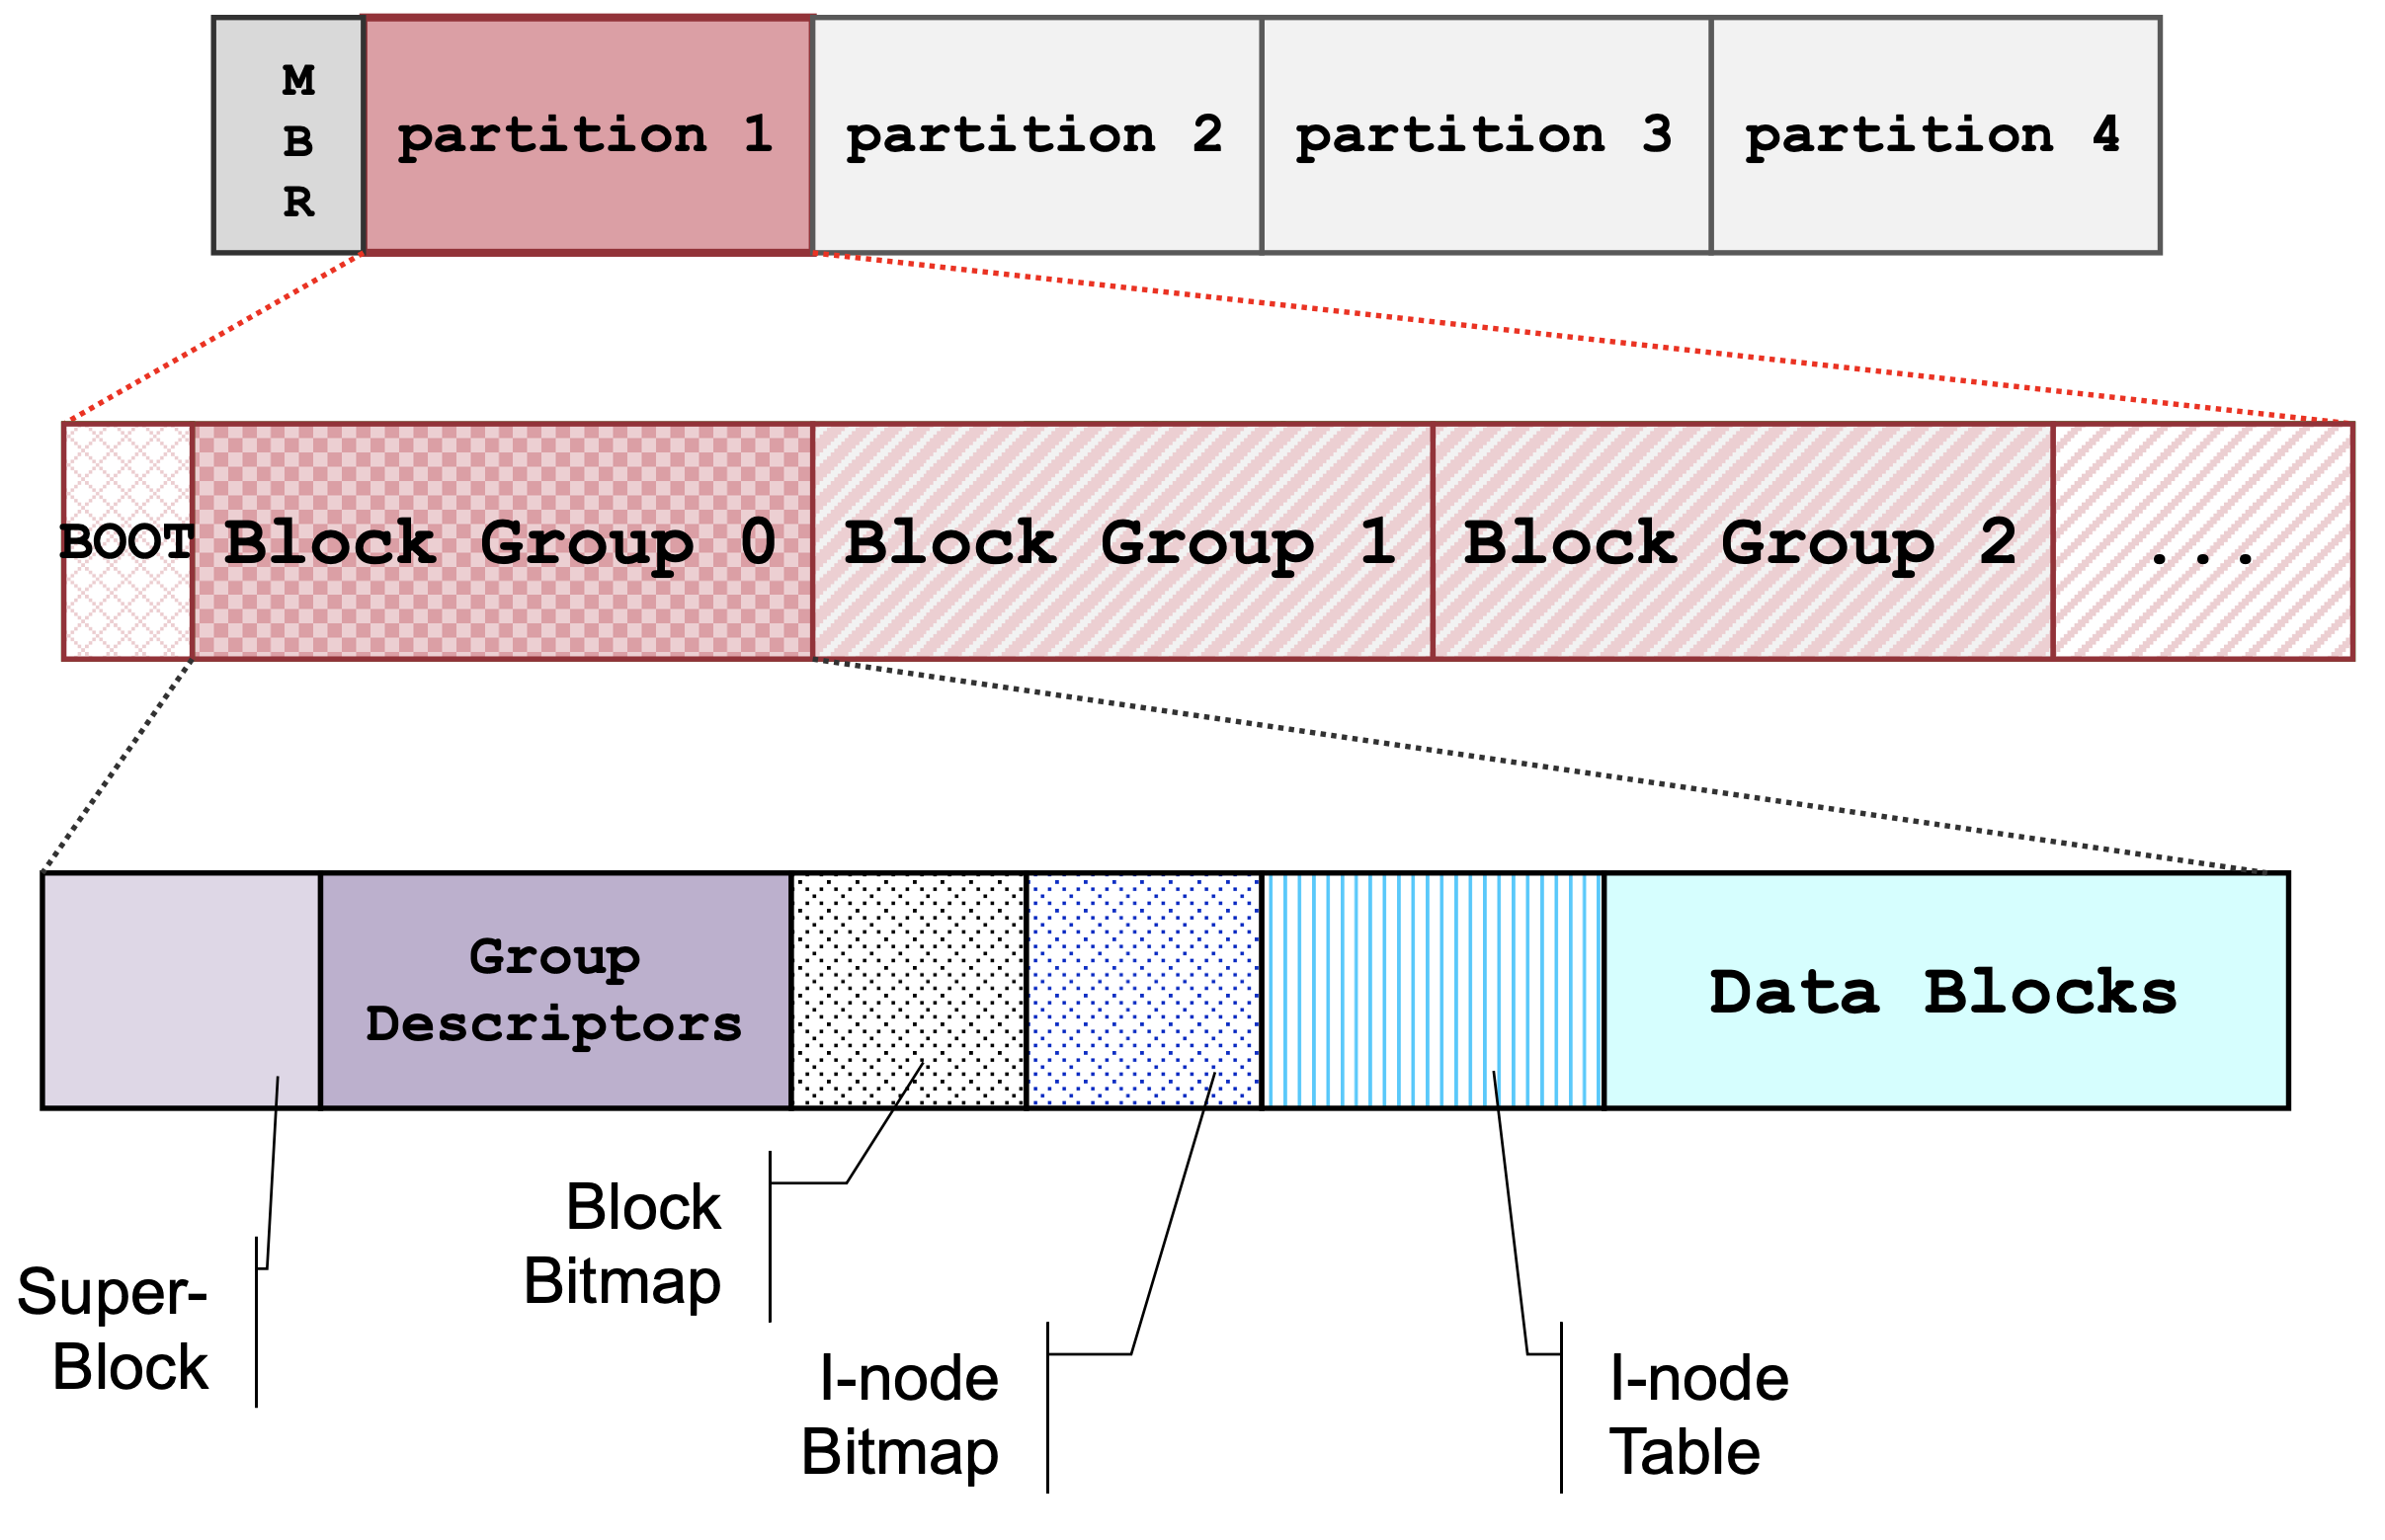
\includegraphics[width=0.24\textwidth]{EXT2/layout}
      \end{center}
    \subsubsection*{Superblock}
      \ull {
        \item Describes entire FS
        \item Total I-nodes, Total disk blocks, etc.
        \item Duplicated in each block group for redundancy
      }
    \subsubsection*{Group descriptors}
      \ull {
        \item Describe each block group
        \item No. of free disk blocks, free I-nodes
        \item Location of bitmaps
        \item Duplicated in each block group for redundancy
      }
    \subsubsection*{I-nodes}
      \paragraph{I-node bitmaps} \noindent
        1 = Occupied, 0 = Free, 1 entry per directory/file
      \paragraph{I-node table} \noindent
        Array of I-nodes of this block group
      \paragraph{I-node structure}
        (also refer to previous page Unix I-node section)
        \begin{center}
          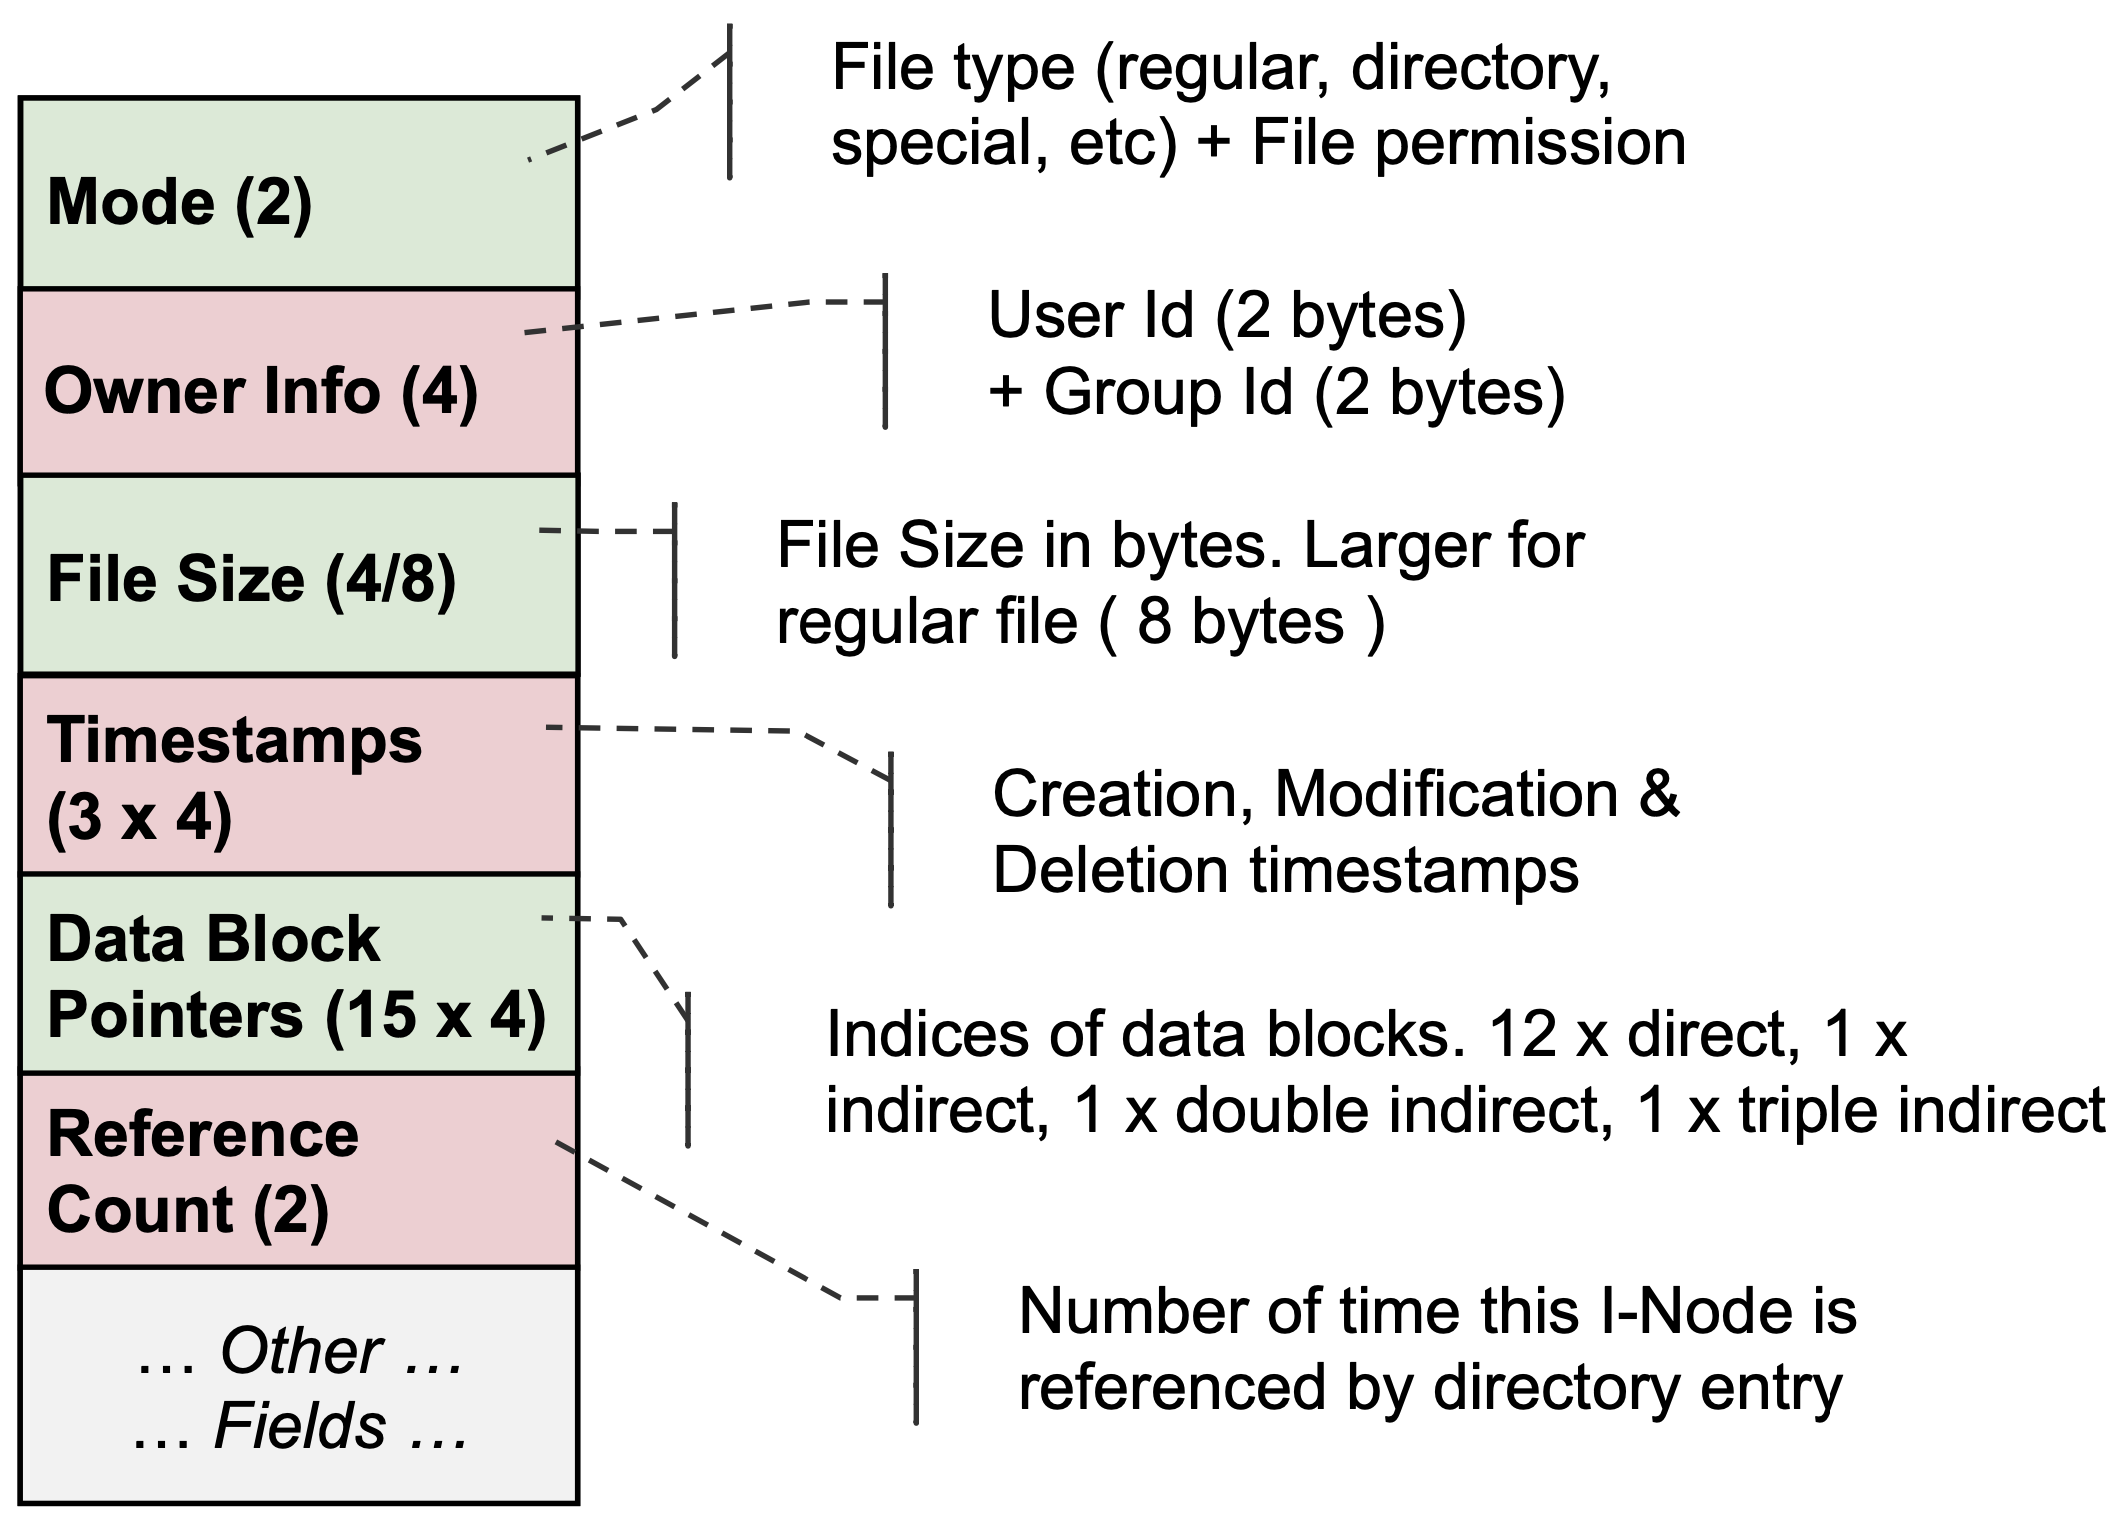
\includegraphics[width=0.24\textwidth]{EXT2/inode_table_layout}
        \end{center}
        \ull {
          \tick Allows fast access to small files (using first 12 disk blocks)
          \tick Flexibility in handling huge file (using single/double/triple indirect blocks)
        }
        \begin{center}
          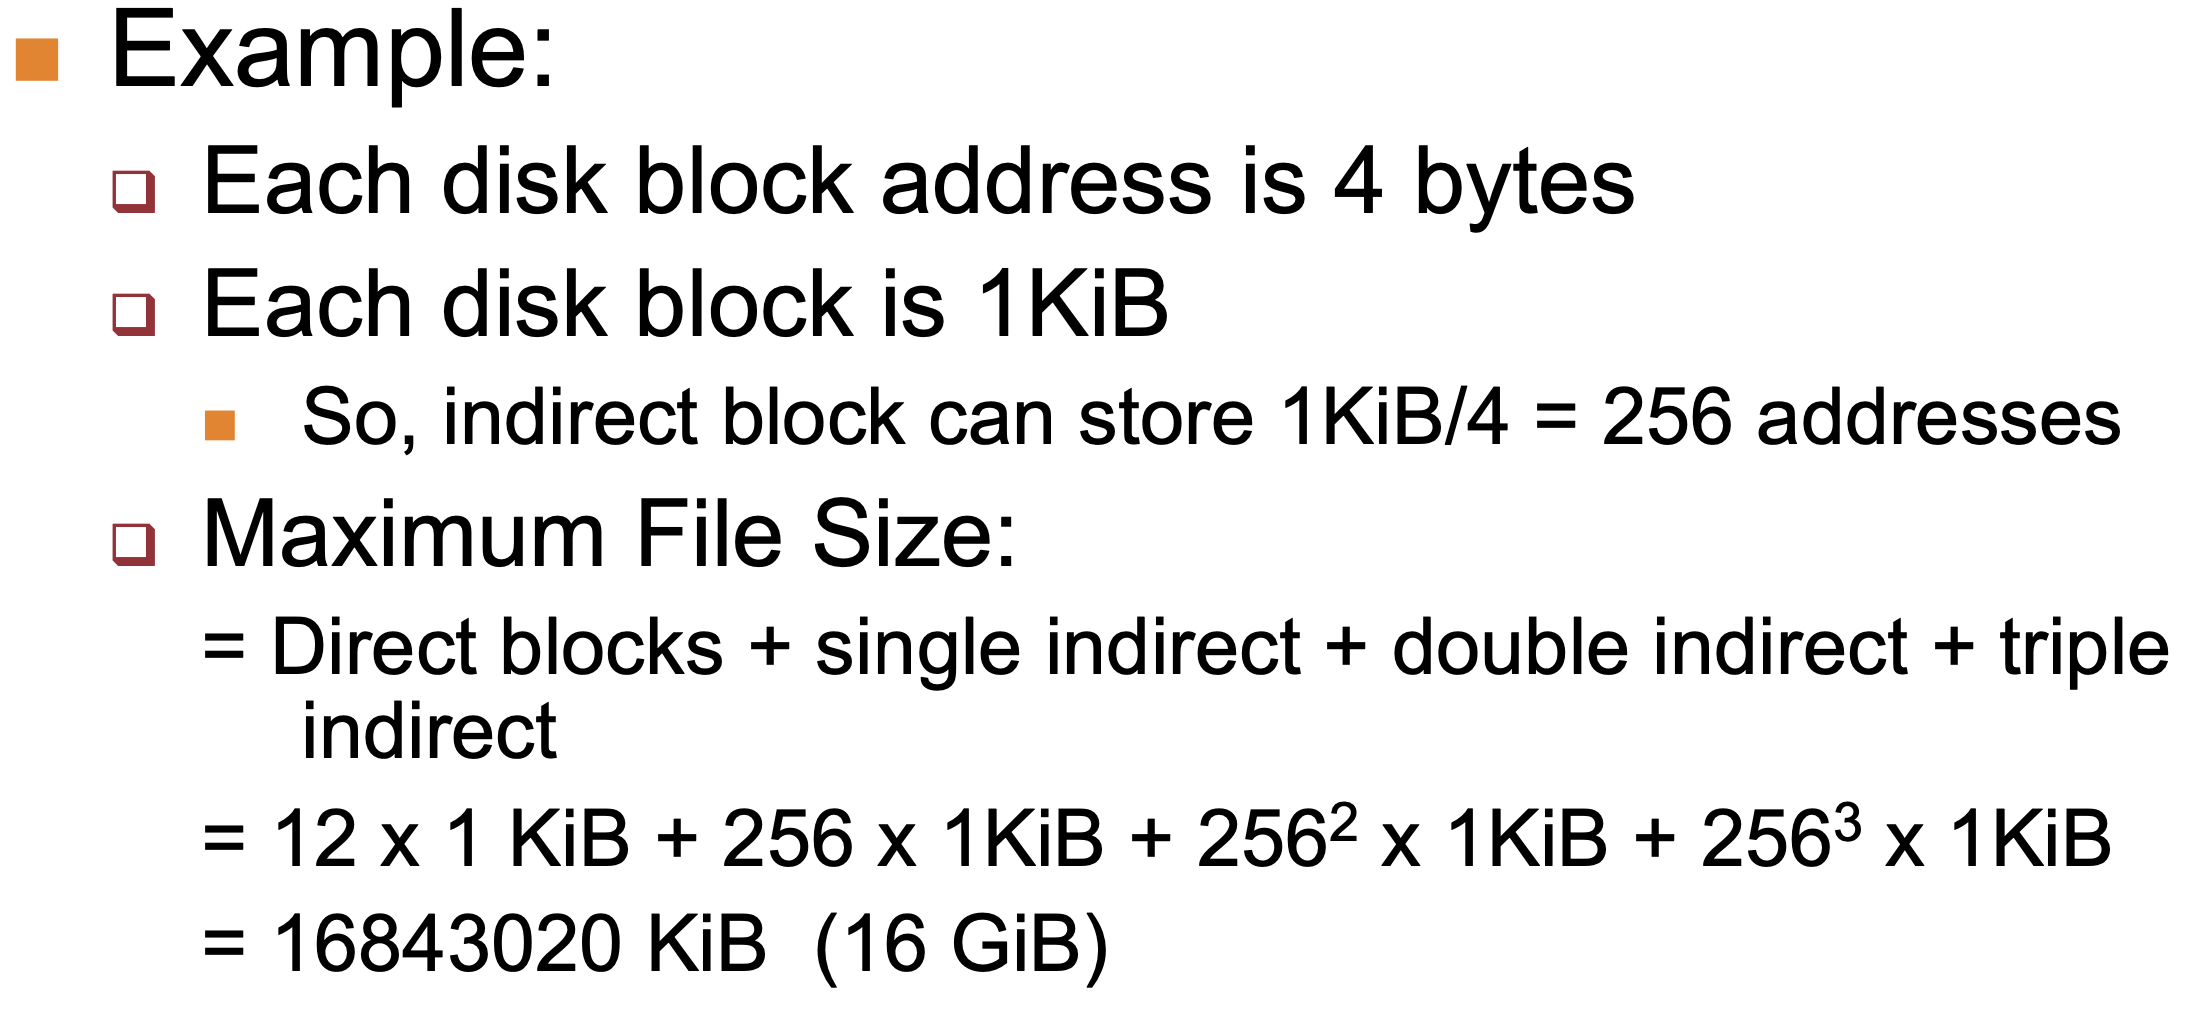
\includegraphics[width=0.24\textwidth]{EXT2/inode_size_limit}
        \end{center}
    \paragraph{\uline{Directory structure}} Data blocks of a directory stores a linked list of directory entries
    \subsubsection*{Directory entry}
      \ull {
        \item Store entry size to locate next entry
        \item File/subdirectory name up to 255 chars
      }
      \begin{center}
        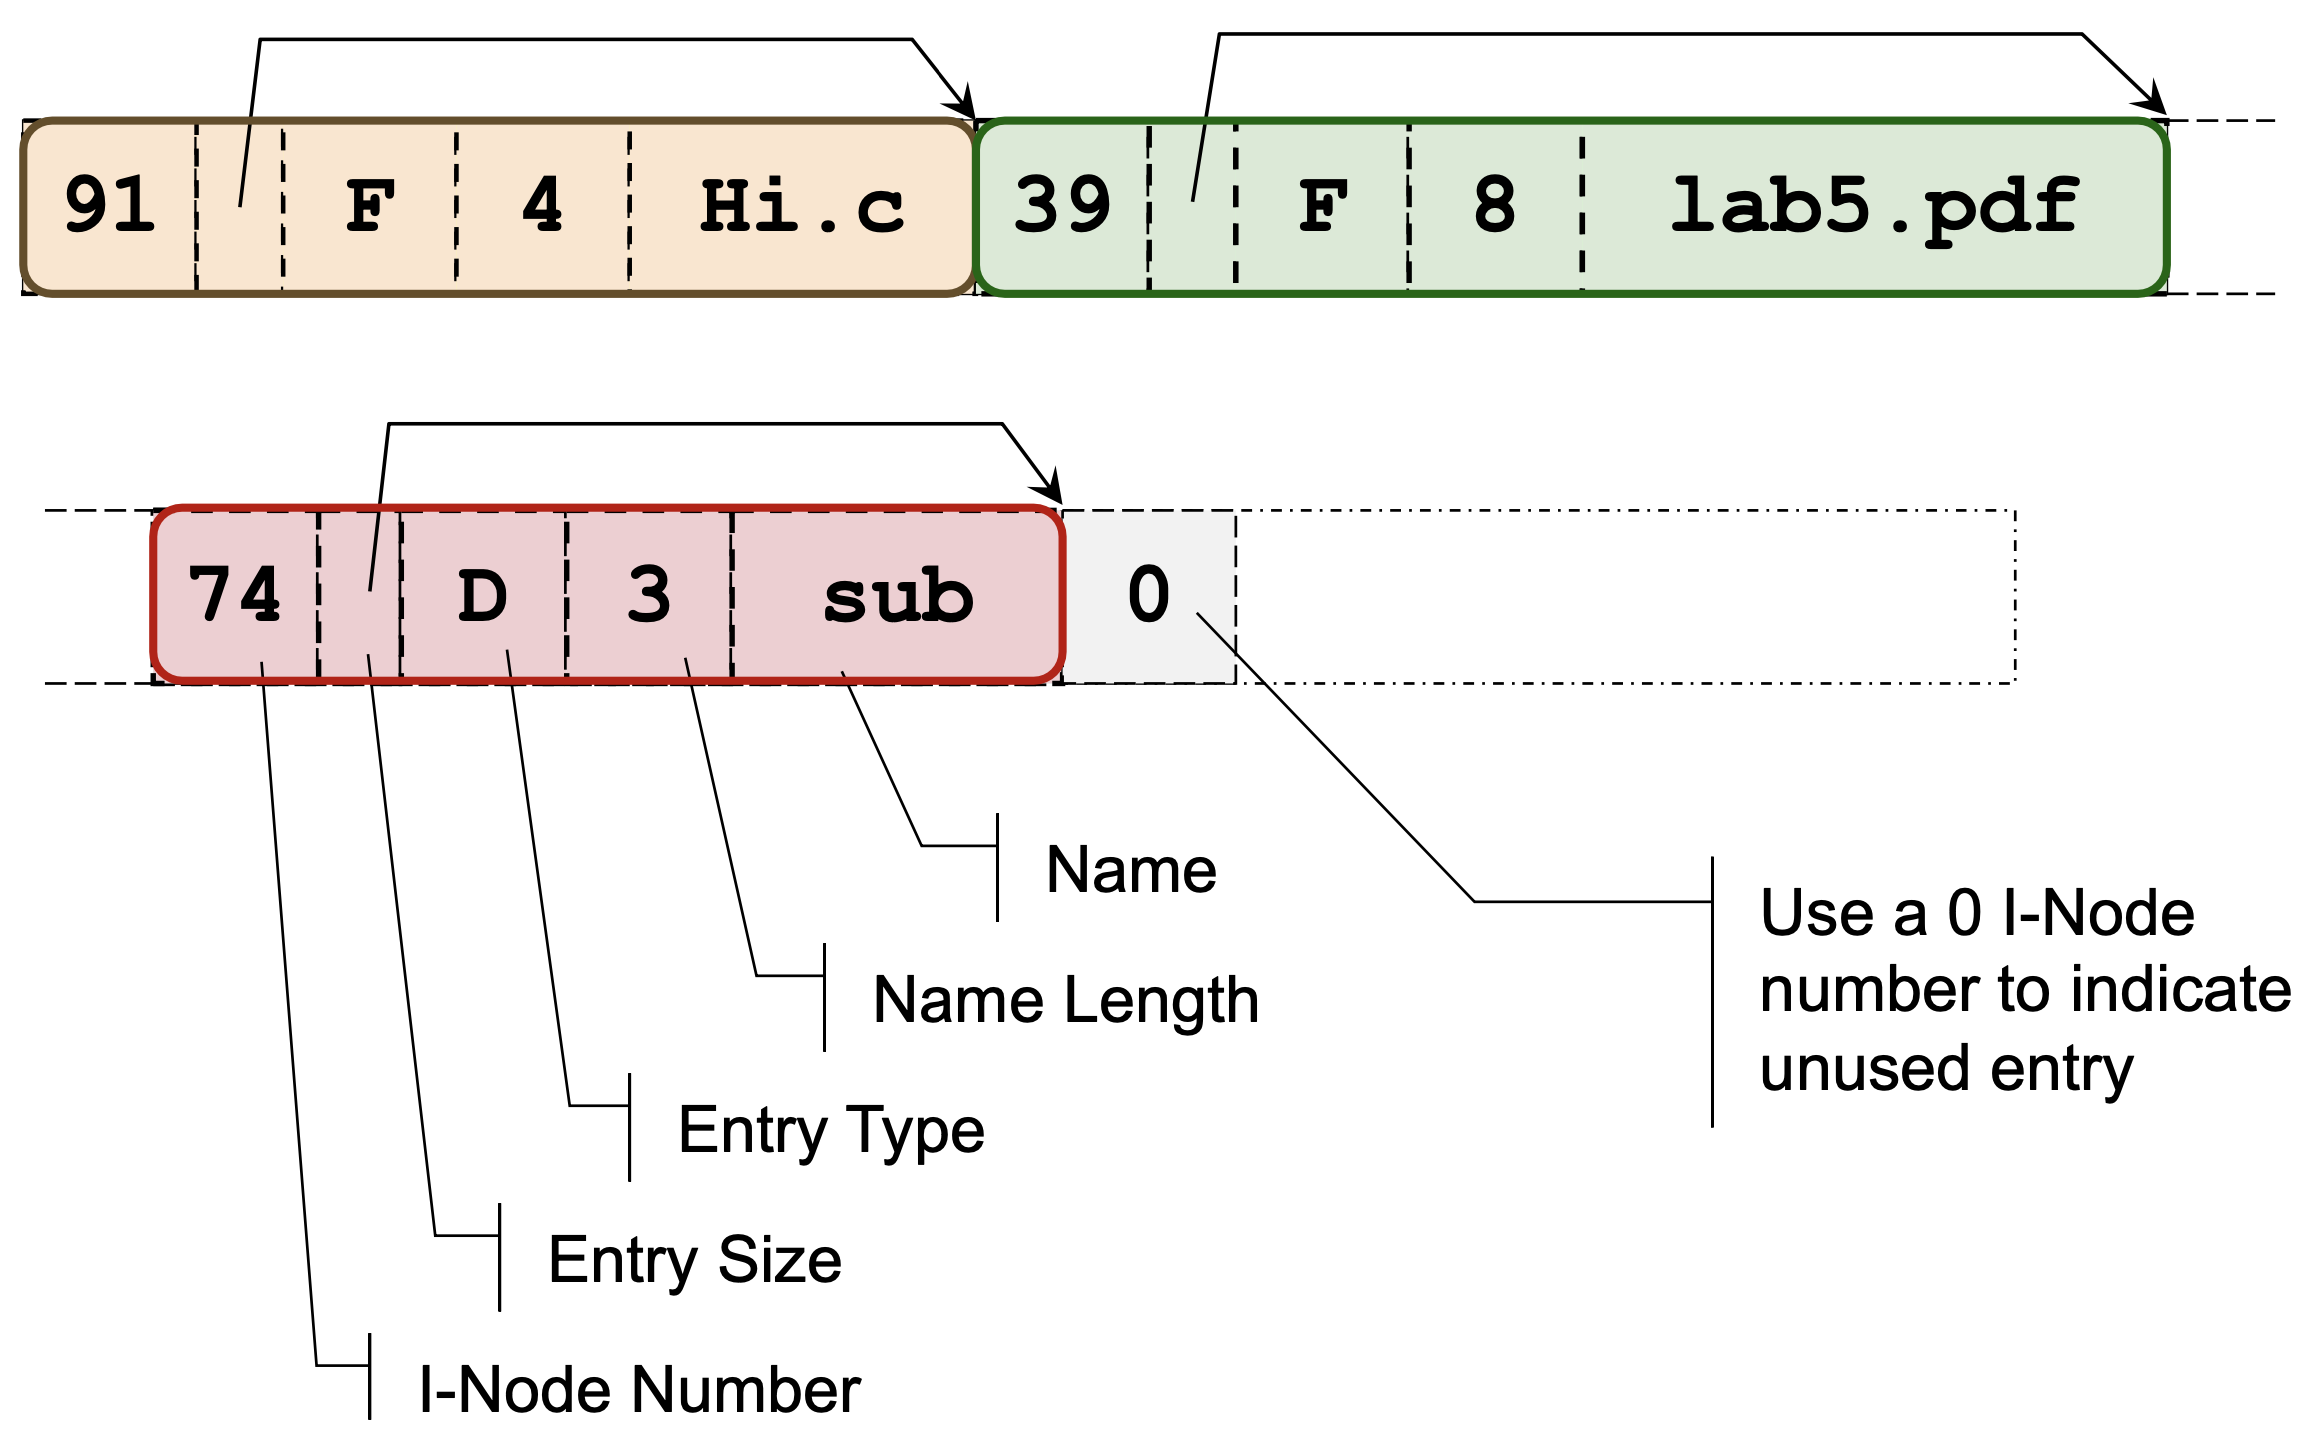
\includegraphics[width=0.24\textwidth]{EXT2/directory_entry}
      \end{center}
    \subsubsection*{File deletion}
      \ull {
        \item Remove its directory entry from parent directory
          \ull {
            \item Point previous entry to next entry/end
            \item Blank record for first entry
          }
        \item Update in I-node and block bitmaps to free
      }
    \subsubsection*{Hard link}
      \ull {
        \item Multiple directory entries point to same I-node
        \item Maintain a I-node ref count, only delete when count is 0 (i.e. all hard links deleted)
      }
    \subsubsection*{Symbolic link}
      \ull {
        \item Only file pathname is stored
        \item Involves a search to locate actual I-node number of target file
        \cross Link can be easily invalidated
      }
  \subsection*{Misc}
    \subsubsection*{FS consistency checks}
      \ull {
        \item Power loss/system crash can render FS in inconsistent state
        \item Windows: \ic{CHKDSK}, or Linux: \ic{fsck}
      }
    \subsubsection*{Defragmentation}
      \ull {
        \item File data can be scattered across many disjoint blocks on storage media, impacting I/O performance
        \item Windows: use software to alleviate problem
        \item Linux
          \ull {
            \item Files are allocated further apart
            \item Free blocks near to existing data block are used if possible
            \item Fragmentation is very low when drive occupancy $< 90\%$
          }
      }
    \subsubsection*{Journaling}
      \ull {
        \item Keep additional info to recover from system crash
        \item Write info and/or actual data inot a separate log file before performing file op
      }
  \subsection*{Other FS}
    \paragraph{Virtual File System} Provides another layer of abstraction on top of existing FS
      \ull {
        \item Allows app to access file on different FS
        \item File ops are translated by VFS automatically to the corresponding native FS
      }
    \paragraph{Network File System}
      \ull {
        \item Allows files to reside on different physical machines
        \item File ops are translated into network ops
      }
    \paragraph{New Technology File System}
      \ull {
        \item Used in WinXP onwards
        \item File encryption, file compression
        \item File versioning
        \item Hard/Symbolic link
      }
    \paragraph{Extended-3/4 FS (Ext3/Ext4)}
      \ull {
        \item Journaling
        \item In-place upgrade from Ext2
        \item Expanded max file and file system sizes
      }
    \paragraph{Hierarchical File System Plus (HFS+)}
      \ull {
        \item Used in Mac OS X
        \item Compression, encryption support
        \item Large FS, file and number of file/folder support
        \item Metadata journaling
      }
\section*{Past questions}
  \paragraph{1920 S1 Q5 (page table size)}
    \begin{center}
      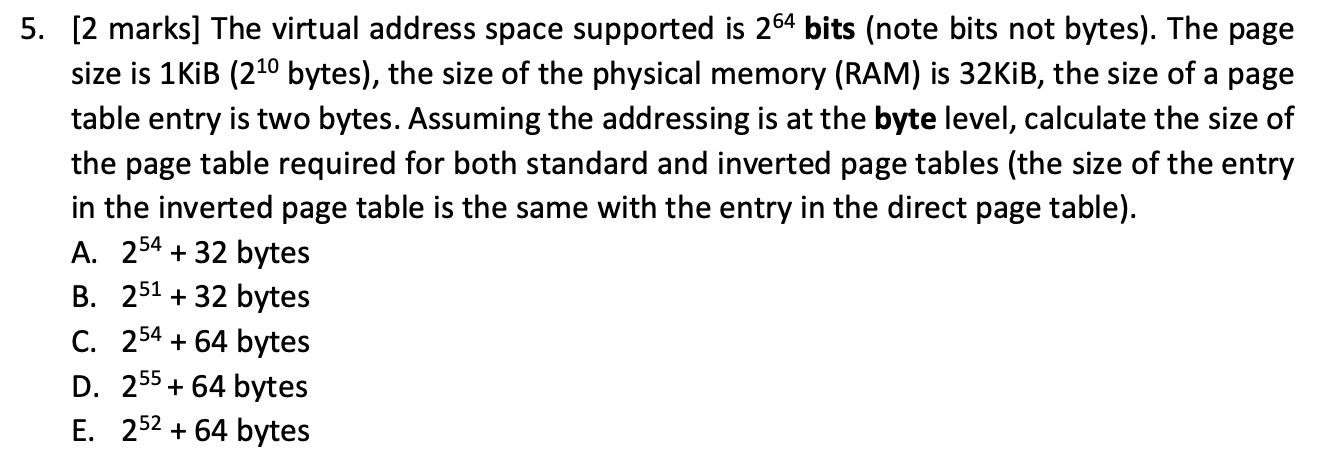
\includegraphics[width=0.24\textwidth]{past_questions/1920S1_Q5}
    \end{center}
    \ull {
      \item Ans: E ($2^{52} + 64$ bytes)
      \item Assuming 8 bits = 1 byte, then $2^{64}$ bits $= 2^{61}$ bytes of addressable memory
      \item 32 KiB / 1 KiB = 32 frames for entire RAM
      \item $32 \times 2$ bytes each = 64 bytes for inverted page table
      \item $2^{10}$ bytes per page, so $2^{61} \div 2^{10} = 2^{51}$ logical pages required
      \item $2^{51} \times 2$ bytes $= 2^{52}$ space for standard page table
    }
\end{multicols*}
\end{document}
